%!TEX option = --shell-escape
\documentclass{article}
\usepackage[utf8]{inputenc}
\usepackage{amssymb}
\usepackage[english]{babel}
\usepackage{graphicx}
\usepackage{wrapfig}
\usepackage[english]{babel}
\usepackage{algorithm}
\usepackage{algpseudocode}
\usepackage{amsthm}
\newtheorem{definition}{Definition}[section]
\newcommand{\norm}[1]{\left\lVert#1\right\rVert}
\newtheorem{theorem}{Theorem}[section]
\newtheorem{corollary}{Corollary}[theorem]
\theoremstyle{remark}
\newtheorem*{remark}{\textbf{Remark}}
\newtheorem{lemma}[theorem]{Lemma}
\usepackage{amsmath}
\usepackage{tikz}
\usetikzlibrary{shapes.geometric, arrows}
\usepackage{geometry}
\geometry{a4paper, top=2cm, bottom=2cm, left=1.5cm, right=1.5cm}
\usepackage{imakeidx}
\usepackage[T1]{fontenc}
\makeindex[columns=3, title=Alphabetical Index, intoc]
\title{Computer and Network Security}
\author{Lorenzo Rossi}
\graphicspath{{Images/}}
\begin{document}
\theoremstyle{definition}

\maketitle

\tableofcontents
\newpage
\part{Parte 1- First Midterm}
\section{Definizioni e basi sulla crittografia simmetrica}
L'obiettivo della crittografia è quello di trasformare i dati in un qualcosa di incomprensibile al fine di garantire confidenzialità e sicurezza. Questa trasformazione deve essere \textbf{reversibile}. Ne è un esempio la crittografia simmetrica in cui si utilizza una chiave che viene utilizzata sia per cifrare che decifrare i dati.
La chiave, come appena detto, serve a cifrare e decifrare i dati e perciò deve essere privata, cioè conosciuta solo da coloro che sono impegnati nella trasmissione. Tuttavia, per permettere la cifratura/decifratura, si necessitano di algoritmi che devono essere noti, cioè pubblici.
L'agoritmo che cifra e decifra viene detto \textbf{chiper}. L'iter che viene eseguito è il seguente:
\begin{itemize}
    \item Il testo non cifrato \textbf{plaintext} P viene cifrato tramite l'algoritmo pubblico (chiper);
    \item Il chiper è una funzione del tipo \(C=ENC(K,P)\) che produce il messaggio cifrato \textbf{chipertext} C ed inviato al destinatario;
    \item Il chipertext viene decifrato dal chiper,che ricordiamo esser pubblico, dalla funzione \(P=DEC(K,C)\) producendo così il plaintext \textbf{originale}.
\end{itemize}
\begin{center}
    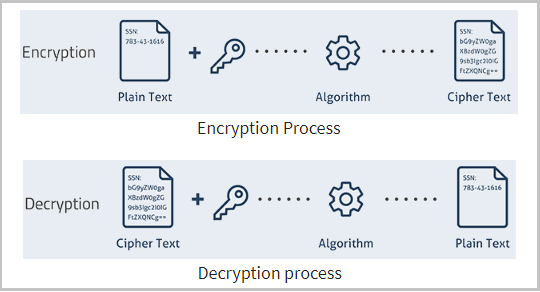
\includegraphics[scale=0.4]{encryption-decryption-diffrences}
\end{center}
\subsection{Substitution cipher}
Il \textbf{substitution cipher} è un algoritmo di cifratura che, preso un plaintext, sosituisce ad ogni lettera un'altra lettera dell'alfabeto. Questo algoritmo è facile da decifrare e poco sicuro poiché è possibile capire la chiave utilizzata (lo schema utilizzato per sostituire le lettere) a mano, ma anche tramite un \emph{frequency analysis} che conta la frequenza delle lettere in una parola. Una volta ottenuta questa frequenza, la si confronta con quella delle parole dell'alfabeto utilizzato e, così facendo, risulta immediato risalire al testo originario.
Un'altra problematica è che questo cipher non preserva la confidenzialità, poiché lo \textbf{stesso} plaintext presenta lo \textbf{stesso} cipher text. Ne sono un esempio le immagini:
\begin{center}
    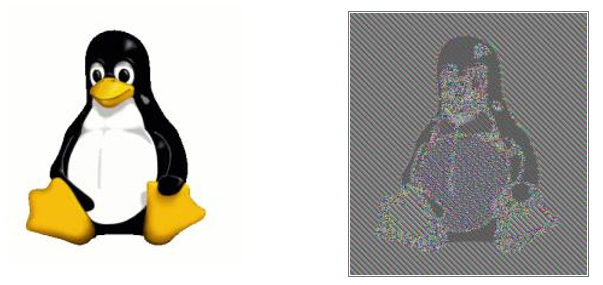
\includegraphics[scale=0.3]{substilug}
\end{center}
\subsection{One time pad-Vernam cipher}
Il \textbf{one time pad} (Vernam cipher) è un algoritmo di cifratura che consiste nella creazione del ciphertext effettuando uno XOR\footnote{l'operazione di XOR funziona come segue: 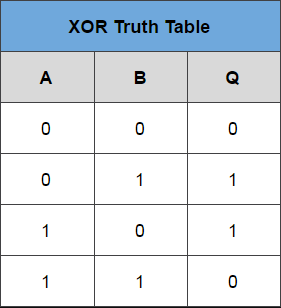
\includegraphics[scale=0.3]{XOR}
} tra il plaintext e una chiave casuale lungua quanto il messaggio da inviare. Definendo \(M\) il plaintext e \(K\) la chiave, possiamo definire l'operazione di cifratura:
\begin{center}
    \(CT=ENC(K,M)=M\bigoplus K\)
\end{center}
A questo punto abbiamo ottenuto il messaggio cifrato \(CT\), per decifrare il cipher text si utilizza l'operazioen di XOR fra la chiave e ciphertext:
\begin{center}
    \(CT\bigoplus K=(M\bigoplus K)\bigoplus K=M\bigoplus (K\bigoplus K)=DEC(K,CT)=M\)
\end{center}
Il \textbf{ Vernam Cipher} è incondizionatamente sicuro, poiché rispetta il \textbf{teorema di Shannon} per cui un cipher è detto sicuro se:
\begin{itemize}
    \item Vi sono tante chive quanti messaggi;
    \item Le chiavi devono essere lunghe quanto il plaintext;
    \item Se le chiavi sono \textbf{casuali};
\end{itemize}
Anche se questo cipher rispetta il teorema di Shannon per la crittografia, risulta:
\begin{itemize}
    \item Assente di integrità (vedere l'esempio sul ciphertext dell'immagine);
    \item Insicuro se le chiavi vengono riusate: l'operazione di XOR cancella le chiavi e lascia i plaintext concatenati in XOR\@;
    \item Le chiavi \textbf{Random} sono difficili da ottenere poiché sono ben diverse da quelle pesudorandomcihe.
\end{itemize}
Riguardo all'ultimo punto, per ottenere una chiave pseudorandomica si utilizza un \textbf{PRNG} (Pseudo Random Number Generator) che è a tutti gli effetti un algoritmo e può risultato buono o sbagliato su diversi aspetti:
\begin{itemize}
    \item Risulta una scelta buona poiché si ottengono proprietà statistiche sull'uscita;\newline
    \textbf{AGGIUNGI ROBA}
    \item Può essere previsto;
    \item Essendo pseudo randomicomo, le chiavi che vengono generati si ripetono con una certa periodicità;
    \item Tutti questi primi 3 aspetti, nella crittografica, sono assolutamenti da evitare, se possibile.
\end{itemize}
Al contrario per ottenere una chiave veramente casuale si utilizzano i \textbf{TRNG} (Truly Random Number Generator) in cui si prendono fenomeni fisici per estrarre la casualità. Ne possono essere un esempio il rumore atmosferico e il rumore termico dei resistori. 
\subsection{One Time Pad-The Attacker}
Ipotizziamo di avere un \textbf{One Time Pad} con un PRNG.Finché l'algoritmo utilizzato per generare le chiavi non è noto sembra essere tutto abbastanza sicuro tuttavia ciò non è possibile poiché, per ipotesi, è pubblico. Inoltre, se ricevessimo due messaggi \emph{M1} e \emph{M2} la situazione cambierebbe:
\begin{center}
    \(M1\bigoplus M2 = (S\bigoplus K_i)(S\bigoplus K_{i+1}) = K_i\bigoplus K_{i+1}\)
\end{center}
Quindi, sapendo che il chipertext è costante, che si utilizza un PSEUDO random generator e che PRNG risulta noto. Per ottenere il plaintext basterebbe effettuare le seguenti operazioni:
\begin{algorithm}
\caption{Break Vernam Cipher-PRNG Version}\label{alg:cap}
\begin{algorithmic}
\State\textbf{Run:} for\((x_i=0;x_i<2^{16};x_i++)\)
\State{\quad \(Z_i = x_i \bigoplus PRNG(x_i)\)}
{\If{\(Z_i == M1 \bigoplus M2 = K_i \bigoplus K_{i+1}\)}{
    \(K_i = PRNG(x_i)\)
}}
\end{algorithmic}
\end{algorithm}
\subsection{Definizioni di Sicurezza}.
Per valutare la qualità di un cipher occorre dare delle definizioni chiave che non possono essere di carattere "assoluto", ma che definiscano con precisione la sicurezza rispetto ad un modello di avversario. Questo perché un cipher può essere sicuro contro un attaccante che è abilitato ad accedere solo al chipertext ma non contro quelli che possono vedere sia porzioni di plain/cipher text. Come convenzione si utilizza un \textbf{modello} rappresentante lo scenario in cui si deve raggiunge l'\textbf{obiettivo}.
A livello internazionale si utilizza come baseline di sicurezza:
\begin{center}
    \textbf{IND-CPA}
\end{center}
In cui:\begin{itemize}
    \item \textbf{IND}: INDistinguishability \newline
    Under
    \item \textbf{CPA}: Chosen PlainText Attack
\end{itemize}

\subsection{IND-CPA Game}
Andiamo ora a definire il modello e l'obiettivo di IND-CPA.Assumiamo la presenza di una vittima ed di un avversario.L'avvrsario è a conoscenza del cipher utilizzato e del plaintext.
\begin{itemize}
    \item \textbf{IND-PHASE}:
    \begin{enumerate}
    \item Scegli \(M_0,M_1\) della stezza lunghezza;
    \item L'avversario invia \(M_0,M_1\) alla vittima;
    \item La vittima prende casualmente uno dei due messaggi con un lancio di una moneta \(M_b,b\xleftarrow[]{} rand(0,1)\);
    \item La vittima genera il messaggio cifrato \(C = ENC(K,M_b)\) e lo invia all'avversario;
\end{enumerate}
    \item \textbf{CPA-PHASE}:
    \begin{enumerate}
        \item[5.] A questo punto l'avversario non sa neanche quale chipertext ha ricevuto e quindi invia i plaintext \(M_0,M_1\) ad un oracolo che conosce sia la chiave e sia il cipher utilizzato.
        \item[6.] L'oracolo risponde con due ciphertext \(C_0 = ENC(K,M_0)\) e \(C_1 = ENC(K,M_1)\)
    \end{enumerate}
    \item \textbf{GOAL}: Se l'avversario deve inviare ulteriori messaggi alla vittima per capire quale sia il plaintext, allora il cipher è sicuro. Altrimenti, il cipher viene detto \textbf{broken}.
\end{itemize}
\subsection{IND-CPA:Conseguenze}
Come abbiamo già detto, un avversario non deve essere in grado di calcolare qualsiasi informazione su un plaintext anche se potessa aver accesso ad oracolo di cifratura. Riformulando:
\begin{center}
    \textbf{Un avversario, dati due plaintexts di stessa lunghezza e dato un ciphertext il quale contiene un messaggio scelto randomicamente tra i due, non dovrebbe essere in grado di distinguere quale dei due sia.}
\end{center}
Le conseguenze di IND-CPA sono che:
\begin{itemize}
    \item La cifratura deve essere randomizzata. Quindi uno stessa messaggio deve restituire diversi ciphertext e quest'ultimo deve essere casuale e quindi indistinguibile.
    \item Se si ripete una sottostringa, deve essere cifrata di due ciphertext differenti.
\end{itemize}
\section{Stream-Cipher e WEP}
Nel mondo reali i ciphers possono essere divisi in due categorie:\begin{itemize}
    \item \textbf{STREAM ciphers}: \newline Deboli: RCA;\newline Forti: Salsa20,ChaCha20;
    \item \textbf{BLOCK Ciphers}: \newline Deboli: DES,3DES;\newline Forti: AES\@;
    \item \textbf{BLOCK ciphers in STREAM MODE}: \newline AES-CTR\@;
\end{itemize}
\subsection{Stream Ciphers}
Lo \textbf{stream cipher} richiede una chiave simmetrica di lunghezza finita scelta casualemente (\(K\)), mentre la chiave utilizzata per la cifratura e la decifratura viene scelto dalla base della chiave simmetrica casuale tramite un algoritmo (\textbf{PRNG(K)} pseudorandom (\textbf{keystream} $K'$)). Per questi motivi, viene detto un cipher one time pad "approssimato".
\begin{center}
    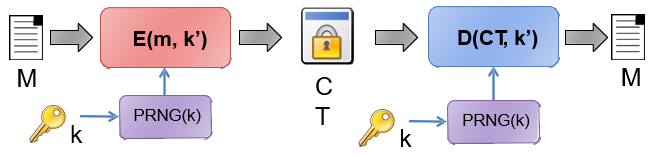
\includegraphics[scale=0.5]{Stream Cipher}
\end{center}
Le funzioni di cifratura e decifratura rimangono invariate:
\begin{center}
    \(CT= ENK(M,M)=M \bigoplus keystream = M \bigoplus PRNG(K)\)
    \(M = DEC(K,CT) = CT \bigoplus keystream = CT \bigoplus PRNG(K)\)
\end{center}
Se si ripete una sottostringa, il chipertext cambia. Tuttavia, se il messaggio viene cifrato due volte, il chipertext si ripeterà dato che il cipher utilizzato è deterministico. Ne è un esempio RC4.\newline
Quindi la problematica è nel fatto che la chiave è statica.
\subsection{Initialization Vectors (IV) in Strem Ciphers}
Al fine di garantire \textbf{sicurezza semantica} si introducono gli \textbf{initialization vectors IV}. Esso è un valore casuale differente per ogni messaggio che garantisce l'unicità del ciphertext. 
In particolare, si IV viene compinato con la chiave dal cipher PRNG (K||V); ne viene fatto lo XOR con il plaintext, ottenendo il chipertext a cui si aggiunge l'initialization vector IV. Quest'ultimo risulterà sempre diverso e la non conoscenza di IV \textbf{NON} è un requisito di sicurezza.
\begin{center}
    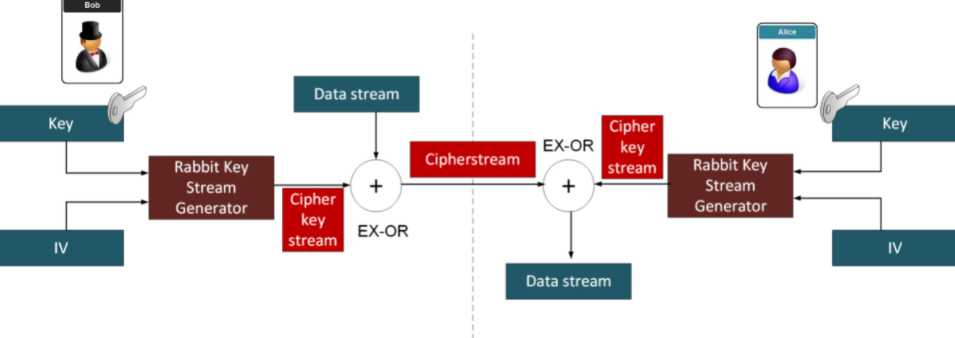
\includegraphics[scale= 0.35]{IVStreamCipher.png}
\end{center}
\subsection{WEP}
L'esempio di WEP è utile a capire perché un buon algoritmo di cifratura non è abbastanza a rendere sicuro un sistema.Inanzitutto, iniziamo con il definire gli obbiettivi preposti da WEP:
\begin{itemize}
    \item Autenticazione:
    \item Integrità:
    \item Confidenzialità;
\end{itemize}
Al fine di garantire questi tre aspetti in Wi-Fi, si scelse di utilizzare come WEP cipher RC4 per generare il keystream.
\textbf{RC4} funziona simile a stream con PRNG:
\begin{itemize}
    \item $ENC(KEY,MSG)= MSG \bigoplus RC4(IV,KEY)$
    \item $Keystream = RC4(IV,KEY)$
\end{itemize}
Quindi, WEP \textbf{per ogni} frame invia un IV differente poiché se avessero inviato un IV per unico keystream si poteva essere poco efficienti in caso di perdita di pacchetti. Inoltre,come  anticipato in precedenza, la trasmissione in WEP di IV in chiaro non è un problema perché da esso non si dovrebbe rompere la sicurezza se si utilizza un buon stream cipher.
Avendo, quindi assunto che RC4 è forte, allora WEP è sicuro finché IV non si ripete mai. Tuttavia vi erano queste problematiche:
\begin{itemize}
    \item Stesso keystream se stessa (Key,IV) e quindi assenza di sicurezza semantica;
    \item Se IV si ripete, la debolezza è pratica.
    \item utilizza di un IV di 24bits;
    \item Generazione di IV lasciato al programmatore.
\end{itemize}
Le conseguenze di queste scelte hanno portato ad una ripetizione dello stesso IV in $2^{24}$ cicli,corrispondenti a 8 ore se ogni frame è di 1500bytes e la rete di 7mbps.
Questa soluzione si rivelò disastrosa e anche se IV veniva scelto in maniera casuale e anche se si sceglieva una chiave di dimensioni maggiori perché il problema era che la lunghezza di IV era troppo corta.
\subsection{Attacchi pratici verso un IV di piccolo dimensioni}
\subsubsection{Attacco Passivo}
Un attacco che si può effettuare in presenza di IV (initialization vectors) di piccolo dimensioni è quello di creare un \textbf{dizionario} formato da:
\begin{center}
    $IV\rightarrow RC4(IV,Key)$
\end{center}
Si utilizzano messaggi noti per recuperare il Keystream nel seguente modo:
\begin{center}
    \begin{equation}
        (MSG\bigoplus RC4(IV,key))\bigoplus MSG\rightarrow RC4(IV,key)
    \end{equation}
\end{center}
I messaggi noti possono essere raccolti anche tramite l'invio di email contenenti grandi allegati. Per proteggersi da questi attacchi si necessita di una \textbf{procedura di autentitcazione}
\subsubsection{IV ripetuti}
Un'altra tecnica è quella di aspettare che un IV sia ripetuto ed in particolare:
\begin{center}
    \begin{equation}
        (M'\bigoplus RC4(IV,key))\bigoplus RC4(IV,key)=M'
    \end{equation}
\end{center}
Come già discusso in precedenza, l'aumento della grandezza della chiave non risolve il problema poiché l'IV mantiene la stessa lunghezza di 24 bits, insufficiente per mantenere un certo grado di sicurezza.
\subsubsection{Attacco ad RC4}
RC4 è l'algoritmo utilizzato da WEP per generare il keystream utilizzato per cifrare i messaggi. Fluhrer, Mantir e Shamir riuscirono a rompere questo algoritmo notando che nel 5\% dei casi la chiave generata da RC4 faceva intuire il valore della chiave utilizzata come argomento di questafunzione. Quindi dimostrarono che, accumulando traffico, era possibile ottenere la chiave segreta simmetrica.
Questo attacco era molto pratico poiché bastava utilizzare il traffico già noto (es. traffico su internet) per ottenere componenti della chiave segreta. Inoltre, si è dimostrato che questo attacco è lineare con la dimensione della chiave.
\subsection{User Authentication}
Non bisogna confondere il concetto di \textbf{autenticazione} con il concetto di \textbf{identificazione}: nel primo, si vuole dimostrare la propria identità digitale (es. email,ID); nel secondo, si vuole mostrare che la propriaidentità digitale è controllata dal proprietario.
Nel pratico il concetto di autentitcazione utente non è facilmente raggiungibile poiché non è possibile collegare l'ID all'identità nella vita reale. Quindi un organo internazionale chiamato NIST SP, fornisce una definizione di autenticazione utente.
\begin{definition}[Autenticazione utente]
L'autenticazione utente è il processo per stabilire la fiducia nelle identità degli utenti presentate elettronicamente a un sistema informativo.
\end{definition}
I mezzi che possono essere utilizzati per verificare l'autenticazione, possono essere i seguenti:
\begin{itemize}
    \item Qualcosa che solo tu conosci: Password,PIN, risposte a domande già note;
    \item Qualcosa che solo tu hai: Smart card, dispositivi fisici come token;
    \item Qualcosa per cui tu sei: dati biometrici come retina, impronta digitale;
    \item Qualcosa che tu fai: come la scrittura e i movimenti del mouse sul computer;
\end{itemize}
\subsubsection{Autenticazione Wep}
L'idea dietro al Wep (\textbf{Wired Equivalent privacy}) non era quella di autenticare gli utenti, ma quella di redigere una lista di chi poteva utilizzare la rete. Tutti gli autorizzati nella rete avrebbero potuto comunicare senza ausilio crittografico, mentre per quelli al di fuori avrebbero osservato solamente i messaggi cifrati. Quindi, la conoscenza di un segreto comune rendeva un utente fidato.
\textbf{L'idea di WEP}
\begin{center}
    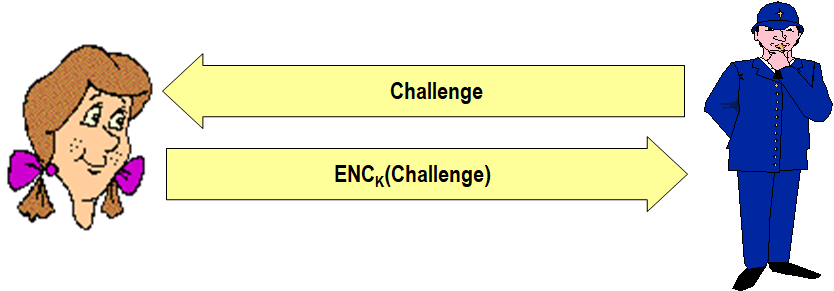
\includegraphics[scale=0.4]{WEPIDEA}
\end{center}
L'idea è quella di utilizzare la stessa chiave del frame anche per l'autenticazione.
\begin{remark}
Questa pratica è \textbf{fortemente} sconsigliata poiché per servizi diversi si devono utilizzare chiavi differenti.
\end{remark}
L'access point invia un valore numerico non cripato come plain text (challenge). L'utente che vuole accedere cripta il valore ricevuto in un modo da dimostrare la sua autenticità. Per ogni utente che arriva cambia la challenge(\emph{sequenza da 128bits}).\newline
Dato che la chiave è pre-condivisa, l'access point sarà in grado di riconoscere se il modo in cui l'utente ha cripato la challenge sia corretto o meno. UNa volta criptata la challenge, l'utente invia all'access point un IV scelto da lui unita alla challenge criptata in XOR con l'RC4(IV,Key).
Gli errori nel fare ciò sono i seguenti:
\begin{itemize}
    \item L'autenticazione WEP è basata sul fatto che la challenge non venga criptata quando inviata dall'access point, ovvero si lascia che il planitext rimanga visibile. Facendo \emph{Chipertext$\bigoplus$ Challenge} si ottiene la keystream. Il grande errore fu usare la stessa chiave nell'encryption e nella challenge. Il WEP in questo modo finisce per implementare un KPA (\emph{Known Plaintext Attack}), in quanto chiunque conosce la challenge può costruire un dizionario composto da \emph{IV-RC4(IV,Key)}. L'autenticazione costituisce un problema per la condifenzialità.
    \item Solo ascoltando una persona fidata per il sistema che conosce la chiave si può riuscire ad aggirare l'autenticazione. L'errore sta nel fatto che IV è deciso dalla macchina di chi manda la challenge criptata, ovvero da chi vuole entrare nel sistema. Cosi facendo, se si esegue:\begin{center}
        $Challenge\bigoplus (Challenge \bigoplus RC4(IV,Key))=RC4(IV,Key)$ \textbf{si ottiene lo stream.}
    \end{center}
    A questo punto, il sistema è sensibile ad attacchi. Posto un MITM(\emph{man in the middle attack}, se esso ascolta IV di un messaggio e si ricava l'RC4 corrispondente, è in grado di entrare nella rete; se a quel punto chiede una challenge all'access point, può scegliere un IV precedentemente intercettato ed entrare nel sistema.\newline
    \textbf{La soluzione a questo problema poteva essere quella di comunicare oltre alla challenge anche l'IV}.
\end{itemize}
\subsubsection{Integrità WEP}
L'idea di WEP per l'integrità era quella di utilizzare CRC-32 come un valore di controllo di integrità così da evitare eventuali manomissioni dei messaggi in WEP.
L'algoritmo \textbf{CRC-32} è un algoritmo di \textbf{error detection} che tiene conto dei bit di partenza tramite bit di parità posti alla fine del messaggio. Quindi, in pratica:
\begin{center}
    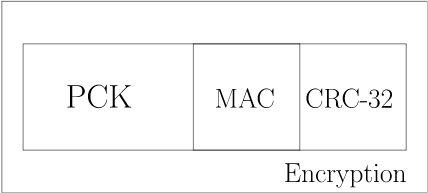
\includegraphics[scale=0.5]{CRCWEP.png}
\end{center}
decisero di includere CRC-32 al pacchetti per poi criptarlo ed inviarlo in rete. Tuttavia, questa scelta si rivelò fallimentare poiché l'algoritmo CRC-32 è lineare rispetto all'operazione $\bigoplus$ e quindi ha permesso attacchi di due tipi:
\begin{itemize}
    \item Modifica dei messaggi;
    \item Iniezione di messaggi.
\end{itemize}
\subsubsection{Modifica del emssaggio}
Supponiamo che un hacker volesse modificare qualche bit del plaintext in WEP.\newline
Quando il messaggio viene mandato, vengono criptati tutti i bit:
\begin{center}
    $C=M|CRC32(M)\bigoplus RC4(IV,Key)$
\end{center}
In questo attacco prendiamo un vettore di bit $\delta$ della stessa lunghezza del messaggio in cui sono settati ad 1 i soli bit che l'attaccante vuole modificare. Quindi, calcoliamo il ciphertext di $\delta$ e calcoleremo il nuovo messaggio:
\begin{align*}
    C'&=C\bigoplus \{ \delta,c(\delta)\}=\\
&=[RC4(IV,K)\bigoplus {M,c(M)}]\bigoplus \{\delta,c(\delta)\}=\\
&=RC4(IV,K)\bigoplus \{M\bigoplus\delta,c(M)\bigoplus c(\delta)\}=\\
&=RC4(IV,K)\bigoplus \{M',c(M\bigoplus \delta)\}=\\
&=RC4(IV,K)\bigoplus \{M',c(M')\}
\end{align*}
Quindi siamo riusciti ad ottenere un messaggio modificato \emph{M'} con RC4 valido.
\begin{remark}
Risulta importante concatenare a $\delta$ anche il suo CRC per ragioni di coerenza con il controllo dei bit di parità.
\end{remark}
\subsubsection{Iniezione del messaggio}
In questo tipo di attacco, l'attaccante necessita ci una coppia IV,RC4(IV,K). Quindi:
\begin{itemize}
    \item Calcola $c(M)$;
    \item Invia $IV,RC4(IV,K)\bigoplus [M|c(M)]$
\end{itemize} 
\subsection{Conclusioni}
Il controllo di integrità deve essere non lineare per non consentire modifiche dei messaggi e deve includere esplicitamente una chiave diversa dato che un crittografica esterna non fornisce garanzie sull'integrità.
\section{Message Authentication: Hash Function}
Occorre evidenziare che \textbf{confidenzialità $\neq$ integrità}. Iinfatti:
\begin{itemize}
    \item \textbf{confidenzialità}: messaggi nascosti. Solo il leggittimo destinatario dovrebbe essere in grado di vedere il contenuto dei emssaggi;
    \item \textbf{Integrità}: autenticità del messaggio. Nessuno dovrebbe essere in grado di modificare un messaggio finché è in trasmissione e la sorgente leggittima dovrebbe essere il solo a forgiare un messaggio.
\end{itemize}
Questi predicati sono corretti finché non si parla di algoritmi AEAD (\emph{authenticatted encryption associated data}.
\subsection{Autenticazione del messaggio con chiave simmetrica}
Il mittente e il destinatario conoscono una chiave \emph{k} dettao \textbf{integrity key}. Questa è una chiave diversa da quella per criptare il messaggio già visto.
L'obiettivo è quello di aggiungere un qualcosa al messaggio che serva da check per l'integrità. Questo qualcosa è il \textbf{TAG}.Il mittente invia al destinatario il messaggio e il tag. Quest'ultimo è una sequenza di bit di lunghezza fissata, di solito più corto del messaggio stesso, generata da un funzione che prende come argomenti la chiave K e il messaggio. In seguito, quando il destinatario dovrà ricevere il messaggio e quindi verificarne l'autenticità, confronterà il tag associato al messaggio e quello che il destinarario del messaggio avrà generato sulla base della chiave K ed il messaggio. Se questo confronto ha buon fine, allora il messaggio è integro.
\begin{center}
    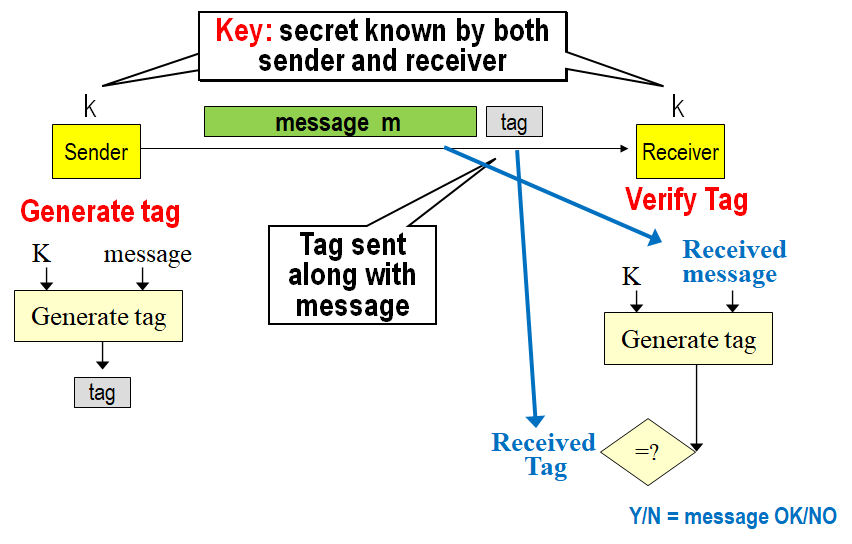
\includegraphics[scale=0.3]{MACSYM}
\end{center}
\subsection{Attacco MITM}
L'autenticazione di messaggio protegge dagli attacchi man in the middle. L'attaccante non può modificare il messaggio considerando le seguenti assunzioni:
\begin{itemize}
    \item $TAG=F(K,m)$ la funzione F è crittograficalmente forte;
    \item L'attaccante vede sia il TAG che il messaggio m, ma non deve essere in grado di risalire a K;
    \item Non può cambiare il TAG senza conoscere la chiave;
    \item Non può cambiare il messaggio utilizzandone un altro che possiede lo stesso TAG.
\end{itemize}
Non è possibile prevenire un man in the middle attack, ma ci si può facilmente accorgere dell'attacco in quanto il tag non corrisponderà. L'attaccante ha solo $2^{-100}$ di probabilità di ricreare il tag giusto dopo aver modificato il messaggio di partenza affinché il destinatario non si accorga dello scambio.
\subsection{Attacco message sppofing}
L'autenticazione di messaggio protegge dal message spoofing,cioè si è protetti dalla ricezioni di messaggi la cui identità non è quella effettiva. Si basa sull'assunzione che la funzione che genera il tag sia crittogaficamente forte e non si può calcolare $F(K,X)$ senza conoscere la chiave segreta.
\subsection{Replay attack}
L'autenticazione di messaggio non protegge dai replay attack: quando si inviano due messaggi uguali, si otterrà lo stesso tag. Questo tipo di attacco non porta problematiche se si è certi che non ci possano essere messaggi uguali.
Per permettere l'invio di due messaggi uguali leggettimamente si utilizzano i \textbf{nonce}. Questi sono delle informazioni che non devono rimanere segrete e che permettono la differenziazione di tutti i messaggi.\newline Queste informazioni aggiuntive vengono inserite nel messaggio così da inglobarle nel TAG e possono essere di tre tipi: \textbf{sequence number},\textbf{random number},\textbf{time stamp}.
\subsection{Nonce: Pro vs Cons}
\begin{itemize}
    \item \textbf{Sequence Number}: la loro problematica riguarda il come gestire i reboot del sistema poiché in ogni avvia del sistema la sequenza ricomincia da capo, ma al contempo si è certi del messaggio che si sta ricevendo;
    \item \textbf{Random Number}: con 128 bit avrei $\frac{1}{2^{64}}$ probabilità di collisione. Tuttavia, non posso tenere traccia dei numeri che sono stati generati. Per risolvere questo aspetto, si potrebbe avere un database in cui si controllano tutti i numeri casuali che sono stati generati, tuttavia le linee da controllare potrebbero essere elevate;
    \item \textbf{Time step}: La problematica è capire come definire l'istante attuale e come prevenire modifica nel gestore dell'orario. Dato che l'orario è può essere impostato manualmente, da un Network Time Protocol (da cui è possibile effettuare attacchi di spoofing) o anche da sistemi di GPS.
\end{itemize}

\subsection{MAC \& Digital Signature}
\begin{itemize}
    \item Nella DS, nessuno può modificare il messaggio ad eccezione del creatore.
    \item Nessuno eccetto il destinatario e il mittente pososno modificare un messaggio autenticato;
    \item MAC e DS hanno l'obiettivo di garantire integrità dei dati/messaggi;
    \item Il MAC (message authentication code) è una forma più debole di una digital signature.
\end{itemize}
\subsection{Definizioni di sicurezza per MAC}
Per la crittografia si era parlato di modello INDCPA per definire la sicurezza. Ora per i messaggi occorre dare una definizione simile.
La sicurezza è imperdonabile e quindi un attaccante non deve essere in grado di creare o modificare i messaggi e ciò implica che l'attaccante nopn dovrebbe essere in grado di estrarre la chiave dalla coppia $\{M,TAG(K,M)\}$.
Formalmente, definiziona la sicurezza contro un modello di attaccante (\emph{Known Message Attack, Chosen Message Attack, Adaptively Chosen Message Attack} a cui gli vengono dati un numero di coppie passate formate da messaggio e tag e un messaggio m. Quindi, l'attaccante non dovrebbe essere in grado di generare un tag valido. La "bontà" della sicurezza viene data in basse alla probabilità di generare una coppia valida e deve essere pressocché nulla.
L'idea di tag minimo per garantire sicurezza è di 96 bit.
\subsection{MAC: Hash function}
Una \textbf{funzione hash} è una funzxione che sintetizza qualsiasi messaggio di lunghezza X in un digest di lunghezza fissa Y. Queste funzioni non sono invertibili.
Per avere un MAC sicuro si ha bisogno di una buona funzione hash (come \textbf{SHA-256}) e di includere il segreto nella hash. A meno che non si possegga una funzione has perfetta (\textbf{random oracle}), ha importanza la posizione in cui si mette il messaggio nella sequenza di bit di ingresso alla funzione hash.
Definiamo il \textbf{random oracle} come un modello black box tale che, dato $X$ in puti, $H(X)$ è un valore veramente randomico. 
Data la proprietà di ripetibilità, a due input uguali corrisponodno due output uguali. Quindi è impossibile avere una funzione has perfetta poiché è è impossibile avere un digest veramente randomico.
Le proprietà di una funzione hash sono le seguenti:
\begin{itemize}
    \item Una funzione hash non è invertibile: dato $Y$, risultato di una funziona hash, è difficile risalire a $X$;
    \textbf{AGGIUNGERE DA APPUNTI}
    \item Una funzione hash possiede la proprietà di resistenza alle collisioni debole: dato $X$, è difficile trovare un altro $X'$ con lo stesso digest;
    \item Una funzione hash possiede la proprietà di resistenza alle collisioni forte: è difficile trovare due generici messaggi che hanno lo stesso digest.
\end{itemize}
\subsubsection{Paradosso del compleanno}
Il paradosso del compleanno ci aiuta a capire la probabilità di collisione, cioè di ripetizione, di due numero:
\begin{center}
    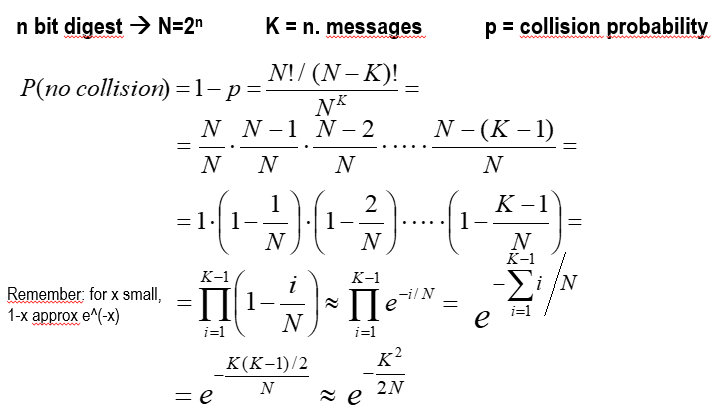
\includegraphics[scale=0.5]{birthdaypdx}
    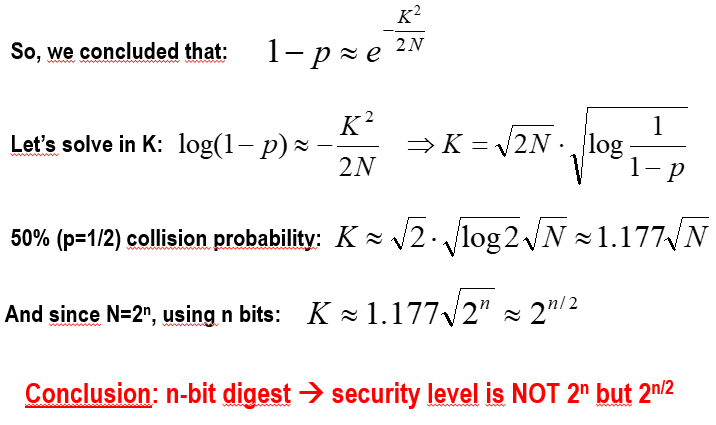
\includegraphics[scale=0.5]{birthdaypdx2}
\end{center}
\subsubsection{Costruzione di una funzione Hash}
\begin{itemize}
    \item \textbf{Segreto come suffisso} Si utilizza la costruzione di \textbf{Merkle-Damgard} per trasformare un set di $k$ bit in un set di dimensione fissata. Ne è un esempio \textbf{SHA-256} che prende $k$ bit arbitrari, li padda aggiungendo 10000 fino ad avere $N\cdot512bit$; negli utlimi 64 viene messo un numero che costituisce la lunghezza del messaggio.\newline
    In generale, si ha un messaggio ed usando il padding e last value si arriva ad avere un messaggio complessivo lungo un multiplo di 512 bit. Questi vengono tagliati in porzioni (chuncks) di 512bit. A questo punto viene preso un IV di 256 bit che è \textbf{DIVERSO} da quello utilizzato nella crittografia e lo si affianca con il primo chunck e , sommandoli, diventano da 768 bit; si applica F e si riottengono 256 bit. questi vengono riattaccata al secondo chunk e così via iterativamente fino alla fine. La \textbf{funzione di compressione} F è il cuore della costruzione della funzione di hash. Se F resiste, allora anche l'iterazione.
    \begin{center}
        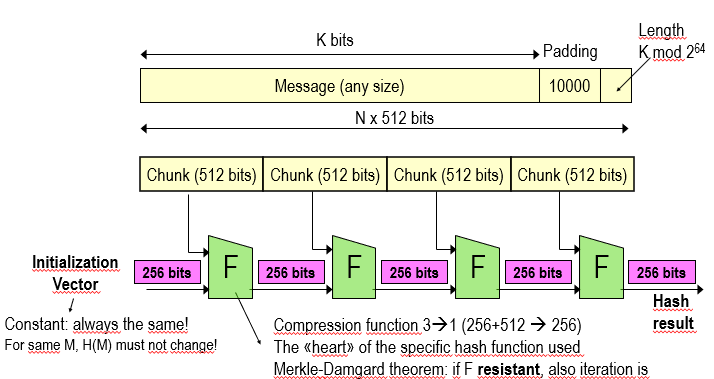
\includegraphics[scale=0.3]{hashConstruction.png}
    \end{center}
    Un attacker potrebbe essere in grado di ridurre la complessità se si pre-calcolasse tutta la parte del messaggio, in modo tale da dover comprirmere con F solo l'ultimo blocco. Questo ridurrebbe la complessità dell'attacco in quanto applicherebbe F una sola volta. Ma comunque è un \textbf{brute force attack}, quindi si dovrebbe comunque indovinare la combinazione corretta di bit.
    \begin{center}
        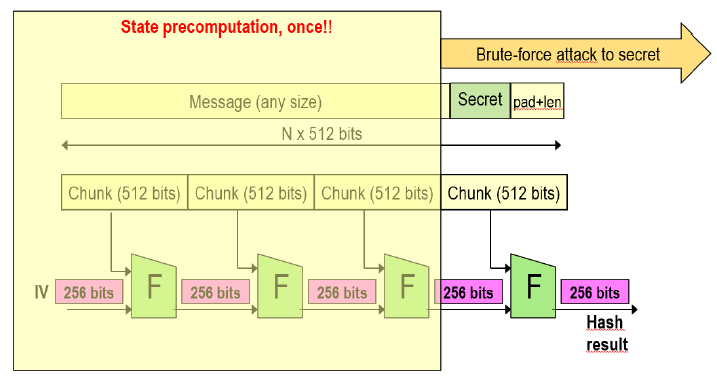
\includegraphics[scale=0.4]{weakSuffix.png}
    \end{center}
    \item \textbf{Segreto come prefisso} Se mettessimo il segreto all'inizio, l'attaccante riesce ad indovinare pad+len e quindi ha violato il sistema. Questo perché oltre il pad+len si aggiunge anche un msg extension alla fine costituito da plaintext arbitrario. In questo caso si crea un extra chunck tale che riapplicando F si ottiene un messaggio valido ma non scritto dall'utente. Non vi è più integrità.\textbf{Message Expansion Attack}
    \begin{center}
        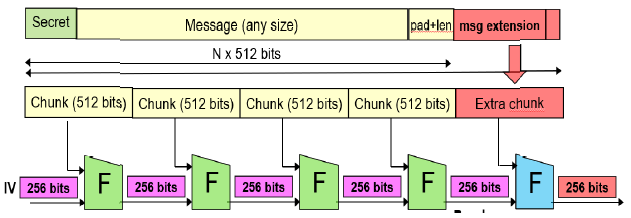
\includegraphics[scale=0.4]{secretPrefix.png}
    \end{center}
\end{itemize}
\subsubsection{HMAC (Hash Based Message Authentication Code)}
L'\textbf{HMAC} costituisce un modo sicuro di aggiungere il segreto nella funzione hash. In particolare, si vuole creare un MAC a partire da un messaggio e un segreto; si applica una funzione hash H sceltra tra quelle esistenti e si calcola:
\begin{center}
    $HMAC_K(M)=H(K^{+}\bigoplus opad||H(K^{+} \bigoplus ipad ||M))$
\end{center}
In cui $K^{+}$ è la chiave precondivisa, estesa alla dimensione di un block grazie all'acquisizione di una serie di 0 di padding (completamento). Si ottenogno così 512 bit di chunk. Fatto ciò si necessita di un secondo segreto che però non viene chiesto all'utente. 
Per ottenere il primo segreto si prende $K^{+}$ esteso e si fa lo XOR con opad (\emph{outerpad, serie di bit composta da 00110110 ripetuti)}.
Per ottenere il secondo segreto si prende la stessa chiave estesa ma si fa lo XOR con ipad(\emph{inner pad formato da 010111100 ripetuti fino a diventare un chunk}.
\begin{center}
    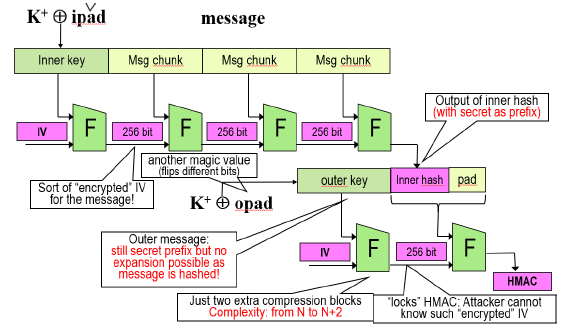
\includegraphics[scale=0.9]{HMAC.png}
\end{center}
Quindi all'utente viene richiesto solo un segreto che viene gestito come segue: si attacca all'inizio del messaggio $K^{+} \bigoplus ipad$; si prende un IV conosciuto e si applica F, ottenendo 256bit che verranno messi in XOR alle porzioni dei messaggi uno dopo l'altro ogni volta riottenendo 256bit e riapplicando F.
Infine, si ottiene un inner hash (vulnerabile) che sarà attaccato con $(outerkey||inner hash|| pad)$. Ora, si esegue la F di IV e outerkey ottenendo 256 bit i quali saranno ricompressi con $inner hash||pad$.
\begin{remark}
\begin{itemize}
    \item Inner hash richiede N compressioni;
    \item outer hash richiede 2 compressioni;
\end{itemize}
La complessità non è aumentata rispetto a prima, ma il risultato è sicuro.
\end{remark}
\begin{definition}[Messaggio Sicuro]
Un messaggio risolta sicuro se ha un'uscita pseudo randomica e non vi sono collisioni.
\end{definition}
\section{User Authentication: Password}
Concettualmente, l'obiettivo dell'autenticazione è quello di dimostrare di sapere una password o un segreto. Tuttavia, si riscontra una differenza tra password e segreto:\begin{itemize}
    \item \textbf{secret key}: è una stringa (true) random di $N$ bit. La probabilità di indovinare una chiave segreta(segreto) è pari a $\frac{1}{2^N}$ con $N$:= numero di bit;
    \item \textbf{Passowrd} è una stringa di N bit in cui i caratteri scelti per comporla non si basano su tutti i caratteri possibili. La conseguenza è che la probabilità di indovinare una stringa è molto minore di quella che si avrebbe con una chiave segreta. Per questo motivo, le password sono stringe a \textbf{bassa entropia}, cioè "poco" casuali. 
\end{itemize}
\subsection{Problematiche delle Password}
Le problematiche delle \textbf{passowrd} sono le seguenti:
\begin{enumerate}
    \item \textbf{Password Overload}: è il riutilizzo della stessa password su siti differenti.
    \item \textbf{Restricted Charset}: l'insieme dei caratteri utilizzati non è completo;
    Per esempio:\begin{equation*}
        1\ bit\rightarrow 256\ caratteri\ possibili;\quad Chiave\ segreta\ da\ 8\ bytes\rightarrow 2^8=64\ bit
    \end{equation*}
    La probabilità di indovinare un carattere è:
    \begin{equation*}
        P_{guess}(s)=\frac{1}{256}
    \end{equation*}
    Ripetuta per 8 caratteri:\begin{equation*}
        P_{totalGuess}(s)=\frac{1}{256^8}
    \end{equation*} Ora assumiamo che il nostro computer abbia una potenza di calcolo di $Rate=66\frac{Mguesses}{s}$. Il tempo medio speso per indovinare la password è pari a :
    \begin{equation*}
        T_{avarege}=\frac{1}{2}\frac{2^N}{Rate}=\frac{1}{2}\frac{1.8\times10^{18}}{6.6\times10^{8}}=4431\ anni
    \end{equation*}
    Nel caso di una Password di 8 bytes, ipotizziamo che l'utente possa utilizzare letteree  numeri lowercase.\begin{equation*}
        1\ byte= 36\ possibili\ valori
    \end{equation*}
    La proboabilità di indovinare una password è pari a:
    \begin{equation*}
        P_{Totalguess}(p)=\frac{1}{N^K}=\frac{1}{36^8}
    \end{equation*}
    Quindi il tempo medio impiegato è:
    \begin{equation*}
        T_{avarege}=\frac{2.8\times10^12}{6.6\times10^6}\frac{1}{2}=5.9\ ore
    \end{equation*}
    \textbf{Come si può vedere la decrescita è esponenziale.}
    \item \textbf{Low Entropy}: Le password devono essere ricordate e quindi non sono randomiche poiché associate ad algoritmi che incosciamente facciamo. 
    L'entropia è la misura di quanto è casuale un qualcosa.
    \begin{remark}
    In un \textbf{Brute Forse Attack} per indovinare $k$ lettere in cui ogni lettera appartienze ad un alfabeto di $n$ lettere. Occorre provare $n^k$ passowrd differenti \textbf{SE} la stringa è stata generata \emph{casualmente}.
    \end{remark}
    Sia $X$ una variabile discreta casuale tale che:\begin{equation*}
        X=\{x_1,..,x_n\} con P=p_i  i=1,..,n\ Probabilit\ uniforme
    \end{equation*}
    \begin{definition}[Entropia]
    \begin{equation*}
        H(X)=-\sum_ip_ilog_2(p_i)
    \end{equation*}
    \end{definition}
    \begin{remark}
    Viene rappresentato in bit e definisce la quantità di informazione osservando l'evento $X$; Per esempio:\begin{itemize}
             \item \emph{lancio di una monenta}:
            \item $x_1=\ faccia\ A\quad x_2=\ faccia\ B\quad p_1=xp_2=\frac{1}{2}$\begin{equation*}
                H(x)=-2(\frac{1}{2}log_2(\frac{1}{2}))=-log_2(\frac{1}{2})=log_2(2)=1
            \end{equation*}
            Quindi l'informazione contenuta in una moneta è di 1 bit.
            Nel lancio di una moneta truccata:$x_1=\ faccia\ A\quad x_2=\ faccia\ B\quad p_1=1 p_2=0$\begin{equation*}
                H(x)=-1log_2(\frac{1}{2})=0
            \end{equation*}
            Quindi vi è total,ente assenza di informazione. Il risultato del prossimo evento è totalmente predicibile.
            \item PIN Code formato da numeri. Ogni numero può assumere 10 valori (0,1,2,..,9) per quattro cifre. Quindi:\begin{equation*}
                p_i=\frac{1}{10}\rightarrow P_{Tot}=\prod_{i=1}^{4}p_i=\frac{1}{10^4}
            \end{equation*} 
            L'entropia vale:\begin{equation*}
                H(x)=-log_2(\frac{1}{10^4})10^4\frac{1}{10^4}=log_2(10^4) bit = 13.28bit
            \end{equation*}
            Nel caso di giorni e mesi:\begin{equation*}
                H(x)=-log_2(\frac{1}{366})366\frac{1}{366}=9 bit
            \end{equation*}
        \end{itemize}
    \emph{\textbf{Altri Esempi Si trovano sui fogli}}
    \end{remark}
    Riassumendo, il \textbf{valore informativo} di $x_i$ dipende da quanto l'evento $x_i$ è inatteso: minore è la proabilità $p_i$, maggiore è il valore informativo di quell'evento. 
\begin{definition}[Information Content]
\begin{equation*}
    Information\ content = funzione\ di\ \frac{1}{p_i}
\end{equation*}
\end{definition}
\begin{definition}[Entropia]
L'\textbf{entropia} è il valor medio dell'\textbf{information content}.\begin{equation*}
    H(X)=E[IC(X)]=\sum_ip_iIC_i=-\sum_ip_ilog_2(p_i)
\end{equation*}
\end{definition}
\begin{center}
    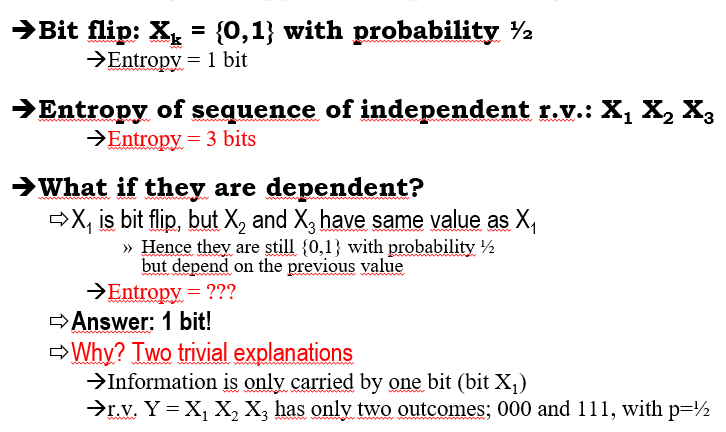
\includegraphics[scale=0.6]{entropy.png}
\end{center}
    \item \textbf{Predictability and Dictionary Attacks}: la scelta delle password è sbagliata e in genere si usano password intuibili dall'umano. I \textbf{dictionary attacks} sono una serie di euristiche di \textbf{attacco brute force} in cui si utilizzano parole comuni, database pubblici di password (ottenuti da altri attacchi andati a buon termine)o dizionari specifici per l'utente che attacchiamo per indovinare la password di un utente. In particolare, per ogni utente si provano tutte le stringe ottenute dai dizionari. Questo è un tipo di attacco che può essere svolto online (facilmente difendibile imponendo un massimo numero di tentativi) o offline (assenza di difesa a patto che si scelga una password forte).
\end{enumerate}
\subsection{Password-Based Authentication vs Challenge-Handshake Authentication - PAP,CHAP}
\subsubsection{PAP-Passowrd Authentication Protocol}
Il \textbf{PAP} è il più semplice approccio di autenticazione possibile. Per dimostrare di conoscere il segreto (passworrd) lo si trasmette in chiaro. In particolare, si invia ID e PASSWORD all'authenticator che possiede un database con scritte tutte le associationi utente/password (ovviamente sono pre-condivise); quest'ultimo controlla la corrispondenza di quesi due valori e in caso affermativo garantisce l'accesso.\newline
Tuttaia questi protocolli hanno delle limitazioni:\begin{enumerate}
    \item Dato che la password e l'id sono trasmessi in chiaro, se qualcuno ascolta mette a repentaglio la sicurezza;
    \item Non vi è protezione da Replay Attack dato che ad un attacker basta ascoltare il messaggio che viene inviato dall'utente all'authenticator per acquisire credenziali valide  per entrare nel sistema;
    \item Non vi è protezione intrinseca sul numero dei tentativi per entrare e quindi si forniscono più tentativi ad un ipotetico attacker per tentare l'accesso.
\end{enumerate}
\subsubsection{CHAP-Challeng-Handshake Authentication Protocol}
Nella autenticazione devo dimostrare di conoscere la password, ma non è necessario che debba dirla in maniera esplicita. Infatti nel \textbf{CHAP} non viene rilevata la password(P), ma la sua funzione di computazione (H(P)), ovvero un prodotto di byte ottenuto a partire dalla password. Assumiamo che:\begin{enumerate}
    \item Questa funzione non sia invertibile: se così non fosse un attacker potrebbe intercettare il messaggio ed eseguire la funzione inversa;
    \item H non deve essere una funzione della solo P, ma deve contenere delle \emph{freshness} (\textbf{nonce,challenge});
    \item H(P) non deve essere ripetibile.
\end{enumerate}
Il CHAP funzione nella seguente maniera:\begin{enumerate}
    \item L'authenticator manda una \textbf{challenge} che \textbf{NON} deve mai ripetersi.
    \item L'utente risponde con l'User ID (\textbf{UID}) e la risposta definita come $H(Challenge,Password,Dati\ aggiuntivi)$;
    \item L'authenticator prende l'User ID (\textbf{UID}) e vede nel databse quale password è associata a quell'utente. Inoltre, conoscendo anche la challenge che aveva mandato, può riapplicare la funzione H da solo per ottenere la rispsota se la risposta dell'utente e quella appena calcolata corrispondono, allora l'utente viene autorizzato ad entrare.
\end{enumerate}
\begin{remark}
Il vantaggio di CHAP è che non deve mai trasmettere la password in chiaro. La funzione non invertibile che viene usata è una \textbf{hash function}.
\end{remark}
\begin{remark}
Ricapitolando:\begin{itemize}
    \item \textbf{PRO}:\begin{itemize}
        \item CHAP protegge dai \emph{replay attacks}, ma bisogna assicurarsi che la challenge non si ripeta mai.
        \item Viene avviato dall'authenticator e quindi un attacker può trovare difficolta a convincerlo a mandare challenge diverse più volte;
        \item \textbf{Challenges Ripetute}: l'autenticazione può essere ripetura durante il tempo di connessione a differenza del PAP che avviene solo una volta all'avvio. Così da verificare più volta l'effettiva identità dell'utente e quindi limita il tempo di esposizione ad ogni singolo attacco.
    \end{itemize}
    \item \textbf{CONTRO}:\begin{itemize}
        \item Il segreto deve essere disponibile in formato \emph{plaintext} e quindi non è possibile utilizzare un database di password crittografate in modo irreversibile.
    \end{itemize}
\end{itemize}
\end{remark}
\subsubsection{One-Time Password}
Il one-time password (OTP) è una tecnica che differisce da one time pad. Si bada sull'idea di migliorare il PAP per avere avere una password diversa ad ogni successfull attempt; questo garantirebbe al sistema una resistanza ai replay attacks. L'idea è quella di memorizzare più password associate ad uno stesso utente, il che però appesantirebbe tropo il DB.
Per ovviare al probelma dellappesantimento del DB si utilizzano le \textbf{hash chain}: catene di shash applicate ad una password di partenza. Questa catena garantisce quindi che la password cambi ogni volta; ogni volta verrà utilizzata una password diversa per entrare generata a partire da quella precedente. Il probme a di questo metodo è che un attacker che ascolta una password poi è in grado di calcolarsi le successive. Una soluzione è usare un hash chain inversa, dove si parte dall'n-esima password generata e si torna indietro. Questa soluzione sembra funzionare, ma estendendola su scala mondiale, ogni singolo utente richiederebbe il calcolo di n hash ne momento di inserimento della password.\newline
Mandare le password al contrare va bene, mabisgno risolvere questo problema computazionale.\newline
\begin{center}
    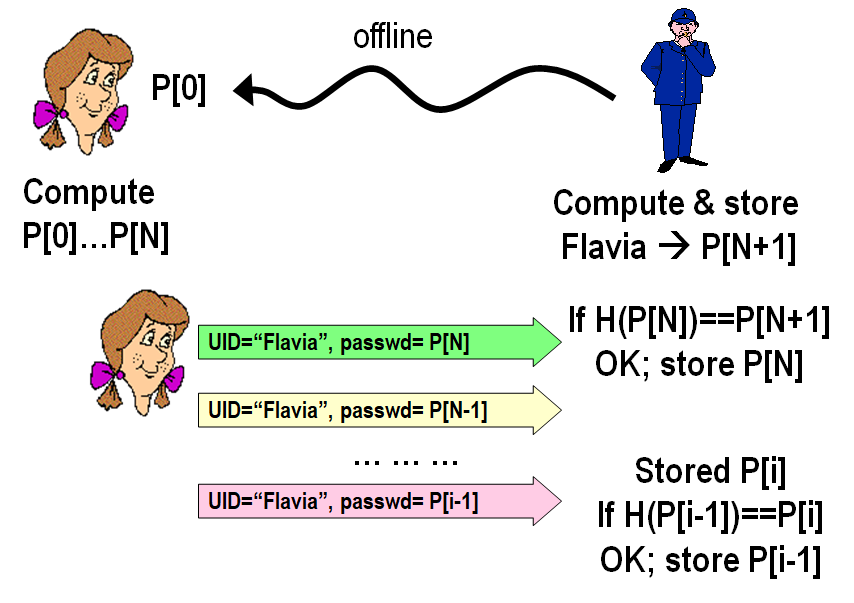
\includegraphics[scale=0.5]{OTP}
\end{center}
Durante la registrazione l'authenticator calcola tutte le password offline fino a $P[n+1]$ e si salva l'ultima. In questo modo quando l'utente vuole accedere fornisce $P[N]$, l'authenticator calcola la successiva applicando la funzione hash, e se corrisponde a quella memorizzata allora l'utente entra nel sistema. L'authenticator sovrascrive a quel punto $P[N+1]$ con $P[N]$ nel suo DB. La prossima v olta l'utente fornirà la password precedente e così via.\newline
Questa soluzione prevede che ogni volta l'utente si calcoli offline sul posto fino al $P[N]$ desiderato. I questo modo effettivamente ad ogni autenticazione verrà eseguita solo una hash da parte del server.
\textbf{Vantaggi}
\begin{itemize}
    \item Ad ogni autenticazione viene eseguita una sola hash;
    \item Il DB memorizza un solo valore per utente;
    \item Robustezza contro attacchi servr-side poiché è impossibile prevedere le password precedenti;
    \item La password può essere trasmessa in chiaro;
\end{itemize}
\textbf{Svantaggi}
\begin{itemize}
    \item Serve un grand valore di $N$ per evitare di finire le password a disposizione;
    \item Vulnerabilità lato client che deve salvarsi il seed delle password o l'intero vettore;
    \item Possibilità di desincronizzazione: se per qualche motivo fallisce una ccesso, si perde la catenta, in quanto l'utente la volta dopo proverà ad entrare con $P[N-1]$ in giù, mentre l'authenticator si aspetta ancora $P[N]$
\end{itemize}
\subsubsection{Autenticazione a due fattori}
Questo tipo di autenticazione si ispira a one time password. Si ipotizza che sia client che server siano sicuri. Ci sono divers requisiti in questo sistema, come un on time authorization token, generato su un device differente o ricevuto su un canale differente. Oltre ciò, il tutto deve essere human friendly cioè si utilizza un hash che trancono le key ad un massimo di 6/8 digit per essere memorizzata.\newline
Ci sono due protocolli:HOTP e TOTP.\begin{itemize}
    \item \textbf{HOTP-HMAC-Base OTP}: Questo protocollo si basa sull'idea di utilizzare un contatore $N$. Sul server e sul client viene memorizzata il segreto $k$ di un utente. Permettendo di fare:\begin{equation*}
        P(N)=H(K,N)
    \end{equation*}
    Questo fa si che non si tratta più di una hash chain (dato che non si applica la hash ripetutamente sullo stesso digest di una password di partenza), ma ogni volta su un bit stream differente. Se un hacker dovesse conoscere $P(N)=H(K,N)$ non può calcolare quello successivo. Inoltre, $P(N)$ può essere calcolata asincronamente senza calcoli ogni volta che vi vuole, dato che occorre avere la chiave di partenza.
    \begin{equation*}
        HOTP(K,C)=Trunce(HMAC-SHA-256(K,C))
    \end{equation*}
    \item \textbf{TOTP0-Time Based OTP}: ogni periodo di tempo viene cambiato il token N per calcolare la password, e non ad ogni accesso come in HOTP. GLia ttacchi a questo tipo di protocollo si basano sul fatto che l'haver possa manipolare il tempo della macchina, così da decidere lui come farlo scorrere per il cambio di token.
    \begin{equation*}
        TOTP=HOTP(K,T)\quad T=(Current Unix Time-T0)/X
    \end{equation*}
\end{itemize}
\subsubsection{CHAP: Mutual Authentication}
L'idea di \textbf{CHAP} è quella di provare ad adattare CHAP ad una autenticazione utente server e viceversa. In generale, si ha che:
\begin{center}
    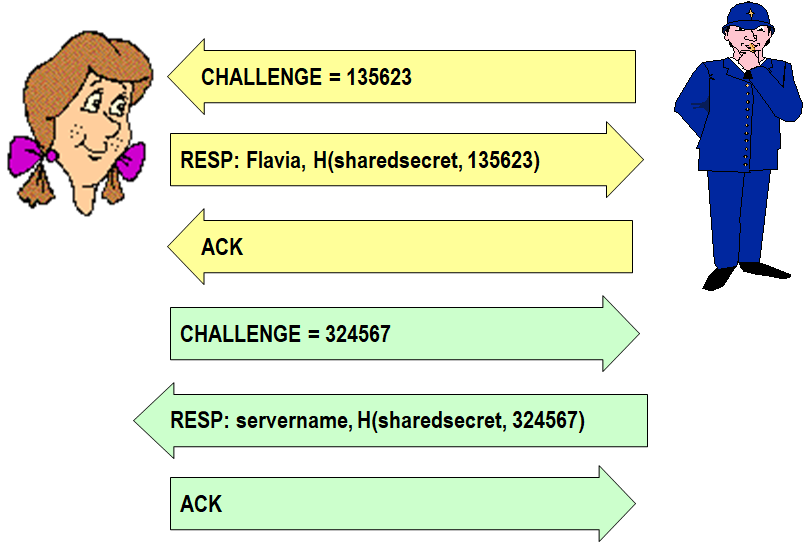
\includegraphics[scale=0.5]{mutual.png}
\end{center}
\begin{itemize}
    \item Arriva la challenge, l'utente risponde con $ID,H(sharedsecrete, challeng)$, l'authenticator manda un ACK;
    \item A questo punto l'utente rimande una challenge nuova; l'authenticator risponde con $ServerName,H(sharedsecre,challenge nuova)$. L'utente manda l'ACK.
\end{itemize}
Siccome non è specificato l'ordine dei messaggi, un hacker può rispondere alla challenge con la stessa challenge, così da ricevere come risposta dall'access point la stessa che dovrebbe dare lui per entrare.\newline
\begin{center}
    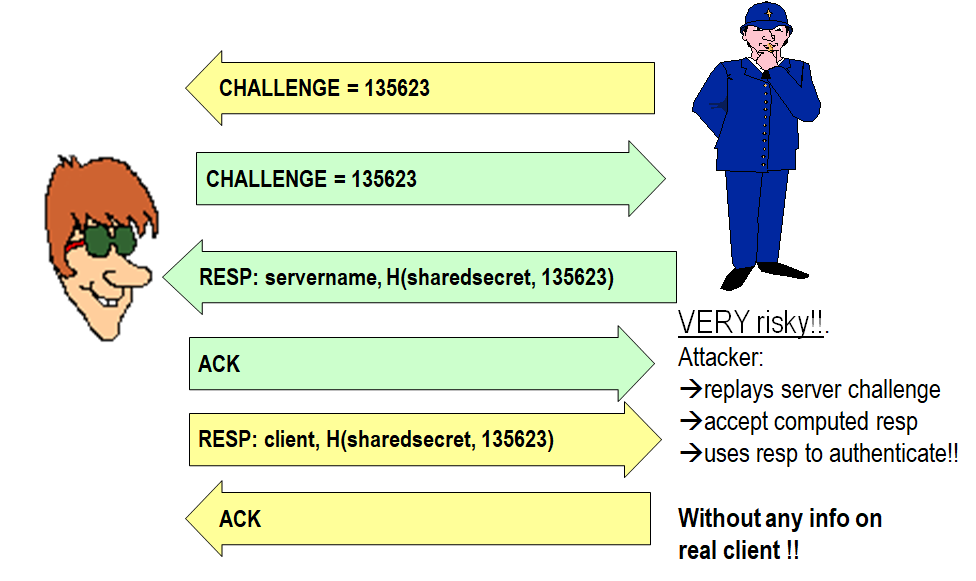
\includegraphics[scale=0.5]{mutualBreak.png}
\end{center}
Questo può accadere perché le due autenticazioni sono unilaterali e non è specificato né in che ordine vanno mandate, né che non possono essere uguali alle challenge. Oltre ciò, il sistema è soggetto al \textbf{reflection attack}: l'attacker si finge acce point e si fa inviare da un utente $ID,C2 e H(secret,C1)$. L'attacker fa finta di non sentirlo e rimanda la challenge appena inviatagli, aggirando di conseguenza i controlli.
\begin{center}
    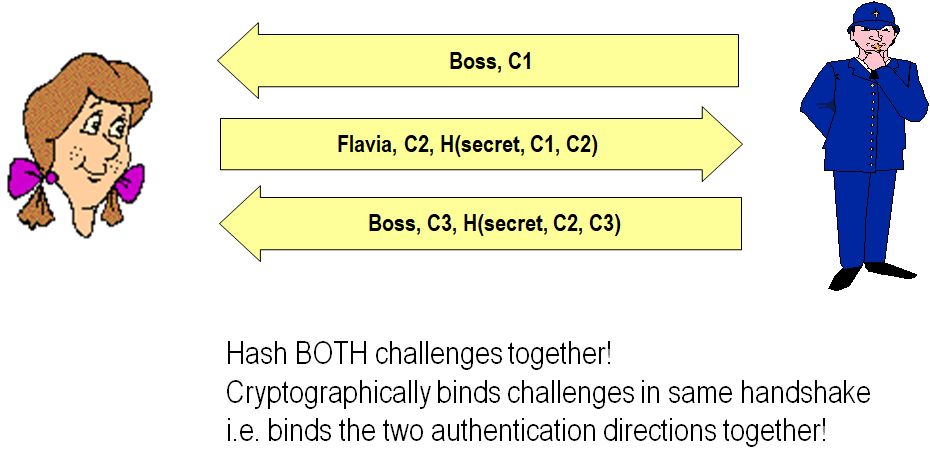
\includegraphics[scale=0.5]{reflectP.png}
\end{center}
Per \textbf{prevenire il reflection attack}, si può procedere nella seguente maniera. Se l'authenticator invia una challenge all'utente, e quest'ultimo propone una challenge diversa che viene inclusa nella funziona hash insieme alla stessa challenge che ha ricevuto. A questo punto l'authenticator rimanda la funzionee hash delle challenge in ordine invero. Quindi, un hacker può sentire le diverse challenge, ma senza aver condiviso precedentemente il segreto e quindi non può calcolare la funzione hash.
Il problema di CHAP, che è stato ideato per autenticazione single side, è che se viene usato in due direzioni, la loro indipendenza espone rischi al sistema. Quindi, occorre renderle indipendenti crittografando due challenge.
\subsection{Chellenge-Response Authentication in Wireless Cellular Systems}
La comunicazione in ambiente wireless di sistemi cellulare si basa sulla comunicazione di tre entità:\begin{itemize}
    \item \textbf{UE}(User Equipment): cipè il mezzo che permette all'utente di connettersi alla rete. In questo caso è la SIM;
    \item \textbf{Serving Network}(SN): è la rete diversa dal provider della SIM che interpella il provider(Home Network) per effettuare la connessione;
    \item \textbf{Home Network}(HN): è la rete del gestore di rete alla quale un utente si autentica.
\end{itemize}
\subsubsection{Autenticazione in 2G(GSM)}
\begin{center}
    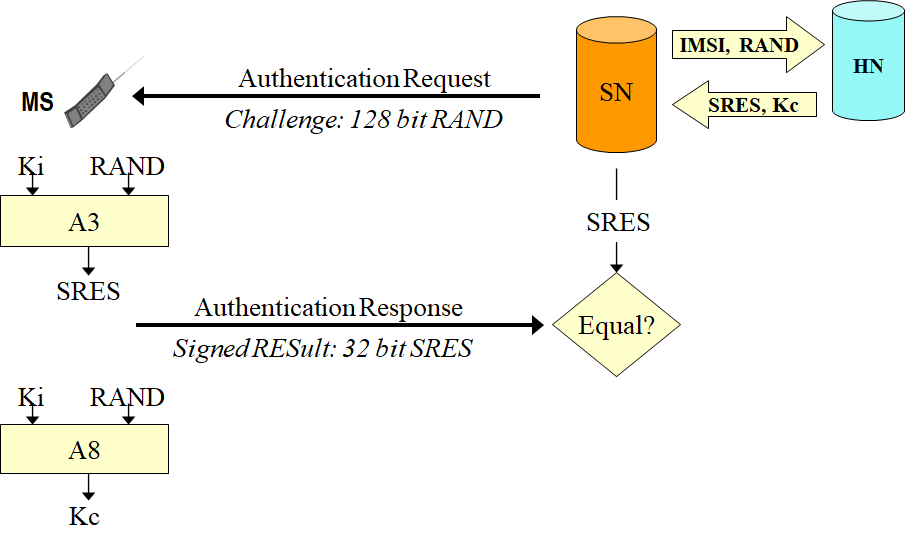
\includegraphics[scale=0.4]{auth2g.png}
\end{center}
Per instaurare la connessione si seguono i seguenti passi:\begin{enumerate}
    \item L'user che si vuole connettere si identifica;
    \item Il server network manda l'\textbf{IMSI}(subscriber identificator, identificatore dell'utente) e \textbf{RAND} challenge all'Home Network;
    \item L'Home Network risponde con SRES (\textbf{$H(RAND,K_i)$ tramite funzione hash A3}) e $K_c$(\textbf{encryption key}) utilizzata nella sessione e generata dinamicamente ogni volta che si vuole autenticare tramite la funzione hash A( a partire da $K_i \ e\ RAND$;
    \item Ora che il Service Network è entrato a conoscenza delle informazioni necessarie allo svolgimento della sessione, manda una authentication request alla MS con una challnge(RAND) di 128 bit;
    \item A questo punto la Mobile Sim crea 32 bit (SRES) a partire dai 128 di challenge che gli sono arrivati facendo ausiliao della funzione hash A3(conosciuta solo dalla sim e dalla Home Network, fornite dal provider). Questo digest di 32 bit è ottenuto a partire da $K_i$ e $RAND$;
    \item Il Service Network conrolla se gli SRES corrispondono e, in caso affermativo, garantisce l'accesso.
\end{enumerate}
\begin{remark}
Il punto di forza è che $K_i$(Identity key- chiave dell'utente) resta nell'Home Network e non esce dal dominio verse il Service Network,grazie alla non invertibilità delle funzioni hash.
\end{remark}
\subsubsection{TRIPLETS}
\begin{center}
    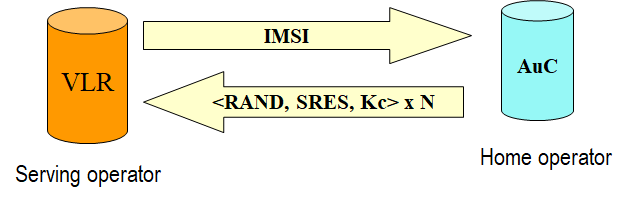
\includegraphics[scale=0.4]{triplets.png}
\end{center}
Un concetto importante nei sistemi cellulare è l'utilizzo di vettori di dati. Si prendono due entità in parti differenti del mondo:\begin{itemize}
    \item \textbf{VLR}: Serving Operator;
    \item \textbf{AuC}: Home Operator;
\end{itemize}
Questa volta, VLR invia solo l'IMSI senza la RAND. AuC risponde con un insieme di vettori di tipo $[Challenge,SRES,K_c]$.\newline la risposta è quindi formata da $N$ triplette di questo tipo. Il vantaggio è che le performance aumentano dato che si mantengono delle triplete in più per le prossime connessioni; inoltre, è che questo mette tutta la sicurezza nelle mani dell'home operator poiché è quest'ultima che gestisce le \emph{nonce}. Quindi, si evita che qualunque hacker possa provare ad attaccare le \emph{nonce} cercando di creare o manipolarle.
\subsubsection{2G:Problematiche}
Dopo l'applicazione di A38(utilizzo A3 e A8 in contemporanea), viene dato $K_i$ e $RAND$ di 128 bit, da cui si ottengono SRES,da 32 bit, e $K_c$, da 64 bit. Il problema fu che in realtà erano 54 bit poiché alla fine non vi erano sempre 10 zeri. Quindi, si perdevano $2^{10}$ combinazioni di sicurezza.
\begin{center}
    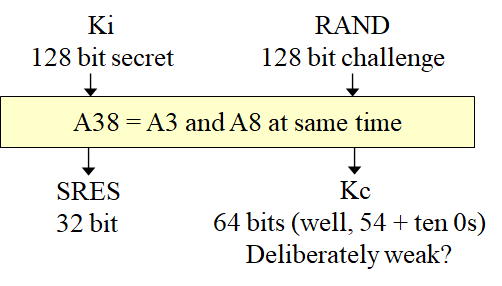
\includegraphics[scale=0.4]{A38.png}
\end{center}
Ogni operatore doveva scegliere come creare la sua funzione di autenticazione: poteva realizzare la sua specifica, oppure utilizzarne una già creata da qualcun altro. Tuttavia, in quel periodo si volle utilizzare COMP128. Questo era il concetto di \textbf{security by obscurity}: si credeva \emph{erroneamente} che nascondere il segreto fosse sicuro.
\begin{remark}
\begin{itemize}
    \item Security by obscurity è fallace. La cosa giusta da fare è lasciar fare algoritmi di sicurezza a chi ne capisce;
    \item Piuttosto che fare un algoritmo privato e chiuso autonomamente, risulta una scelta migliore renderlo aperto e pubblico così che chi è componente può testarlo evidenziandone difetti e pregi;
    \item Una ulteriore problematica del 2G è l'assenza di mutual authentication. Quindi era possibile fingersi una BS (Base Station) fittizia.
\end{itemize}
\end{remark}
\subsubsection{3G(UMTS),4G(LTE),5G}
I protocolli di rete 3G,4G,5G utilizzano il mutual authentication protocol e gli algoritmi sono pubblici (al contrario de 2G). 
\begin{center}
    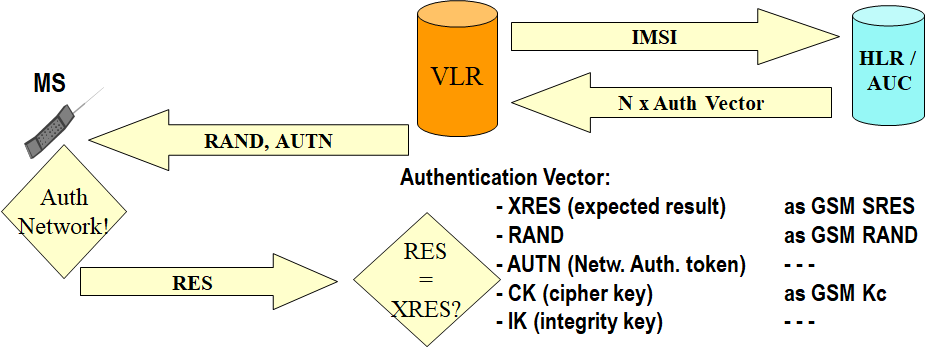
\includegraphics[scale=0.4]{2g3g4g.png}
\end{center}
In qesti nuovi sistemi compaiono nuovamente \emph{MS,VLR,AUC} ed il procedimento è il seguente:\begin{enumerate}
    \item Un MS si connette;
    \item VLR manda IMSI all'Home Network;
    \item HLR manda al VLR delle quintuole che contengono:\begin{itemize}
        \item RAND(Challenge);
        \item XRES: il risultato atteso della CHAP type authentication;
        \item CK: cipher key;
        \item IK: integrity key;
        \item AUTN:\emph{network authentication token}, serve a pìrovare che la rete sia autentica per la mutual authentication;
    \end{itemize}
    \item VLR rimanda quindi a MS: RAND, AUTN;
    \item MS risponde con res per provare che è autentico una volta che riceve un AUTN.
\end{enumerate}
\paragraph{MS Authentication}
\begin{center}
    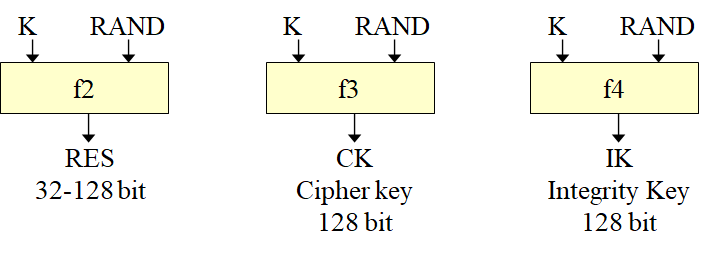
\includegraphics[scale=0.4]{msauth.png}
\end{center}
VLR manda il token che assicura l'autenticità della rete sulla base di una challenge che lui stesso ha generato. Secondo le regole visto fino ad ora non si può provare di essere autentici a meno che non sia l'opponente a creare la challenge.
\subsubsection{Network Authentication - SEQ as Nonce}
La nonce può essere una challenge, una sequenza o un time stamp. Si prende per questo esempio un time stamp ed ipotizziamo che MS e VLR siano in possesso di un GPS e che il tempo non sia attaccabile. Se MS conosce il tempo, in realtà non serve nel time stamp mandare la nonce poiché è già a conoscenza di che ore sono. Considerando che conosce già il riferimento temporare gli basta la risposta di VLR. VLR, quindi, provvede a rispondere diretto con $H(timestamp,secret)$. Usando quindi un secure time reference, è possibile effettuare mutual authentication con un solo messaggio.\newline
Nel caso in cui volessimo fare la stessa cosa con una sequenza di numeri:\newline
MS manda una nonce a VLR ed esso risponde con $AUTH(K,NONCE)$.  Vi è un contatore nella sim chiamato SQN-MS che aumenta ad ogni autenticazione; così quando il VLR manda la sua richiesta di identificazione ad MS, deve anche mettere quanto gli risulta che sia il contatore. In questo modo se MS riceve un contatore minore sa che non si deve fidare.SQN-MS è sincronizzato con SQN-HE quindi, un altor contatore nella home network. Alcuni attacchi si basano proprio sulla desincronizzazione di questi due. In particolare: la sim dell'utente conosce SQN MS; quando VLS manda il suo SQN che proviene da HN, l'utente deve controllare che $SQN=SQN-MS+1$. Se corrisponde, allora può fidarsi della rete.\newline Anche in questo caso con un solo messaggio ci si può assicure che la rete è sicura.
\subsubsection{Formato AUTN}
\begin{center}
    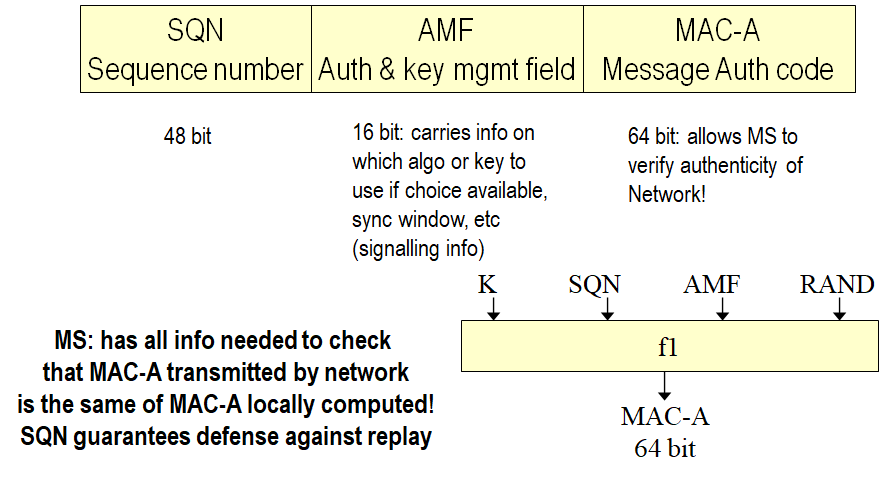
\includegraphics[scale=0.5]{AUTNFORMAT.png}
\end{center}
SQN è il sequence number formato da 48 bit. Attaccati ci sono 16 bit di AMF che rappresenzato quale algoritmo è stato utilizzato e quale finestra di sincronizzazione. Infine, ci sono gli utlimi 64 bit di MAC-A che sono costituiti nel seguente modo: si mettono insieme in una funzione di criptaggio f1 SQN,RAND,K,AMF(informzioni dell'algoritmo). Ed infine, tramite gli utlimi 64 bit, MS può testare l'autenticità della rete.
\subsubsection{Sistema Sfruttato 3G e 4G}
La prima volta che un utente si connette alla VLS, al MS viene inviato un TMSI(temporary MS identifier) che viene allcoato dinamicamente alla prima connessione. Alla prossima autenticazione non verrà utilizzato l'IMSI, ma quel TMSI. Esso è importante perché cambia ogni volta e quindi non è tracciabile. Siccome, vedendo la SQN, un eavesdropper potrebbe discriminare e rintraccia l'utente si masschera con una chiave anonima, si esegue SQN xor AK.
L'AK di 48bit viene generato tramite l'applicazione di una funzione f5 insieme ad un valore randomico ed una volta inviato il pacchetto, per ritrovare SQN viene rieseguito lo xor con AK. Altro passaggio importante è l'esecuzione della funzione f4(SQN,K,RAND,AMF)=MAC-A; verrà controllato con MAC-A inviato precedentemente.
\subsubsection{Generazione chiavi da un segreto}
Per generare infinite chiavi da un solo segreto, si crea un global secret chiamato S, unico. Ogni volta che arriva un nuovo user crea H. In questo modo si ha la sicurezza che nessun utente nel sistema abbia una stessa password, e analogamente quando ne arriva uno nuovo gli viene affidata la sua $K_i$ senza eseguire contorlli su tutte quelle già fornite.
\section{RADIUS}
\textbf{RADIUS} è un protocollo client-server di livello applicativo che utilizza UDP per gestire su larga scala di Access Point eterogenee. In particolare, deve gestire:\begin{itemize}
    \item molteplici NAS (\emph{client});
    \item molteplici servizi di accesso;
    \item Autenticazione e assegnazione della configurazione specifica del servizio.
\end{itemize}
\begin{center}
    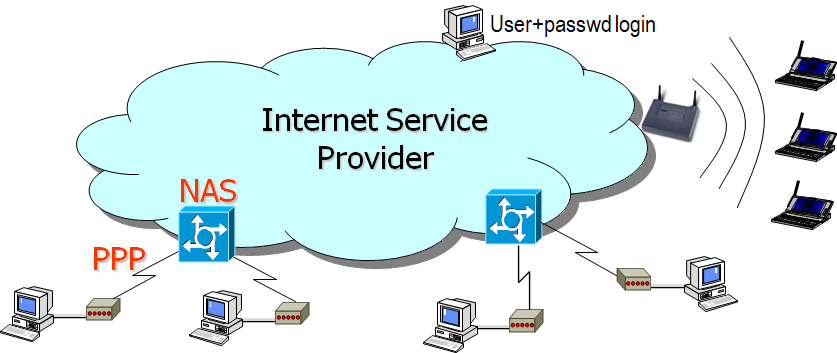
\includegraphics[scale=0.5]{Radius1.png}
\end{center}
La solutione ottima è ottenuta gestendo un DB per ogni singolo utente. In particolare:\begin{enumerate}
    \item L'utente invia gli attributi dell'autenticazione al NAS. \textbf{Assenza di RADIUS};
    \item Il NAS inoltra la richiesta di accesso al server RADIUS;
    \item Il server RADIUS risponde OK,NO, Challenge peer alcuni tipi di autenticazione;
    \item NAS notifica l'utente se può entrare o meno. \textbf{assenza di radius};
\end{enumerate}
\begin{center}
    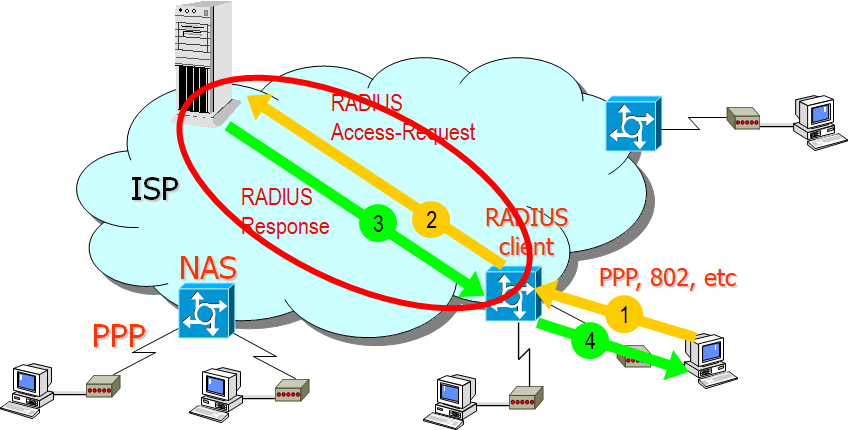
\includegraphics[scale=0.5]{RADIUSW.png}
\end{center}
\begin{remark}
\begin{itemize}
    \item \textbf{PPP:=}point to point protocol;
    \item RADIUS server (AuC) e client (\textbf{NON} RADIUS Client)conosce il vero segreto;
\end{itemize}
\end{remark}
\subsection{RADIUS: AAA Protocol}
Il protocollo Radius è detto protocollo AAA poiché permette di centralizzare:\begin{itemize}
    \item \textbf{Autenticazione}: verifica di chi dico di essere;
    \item \textbf{Autorizzazione}: verifica se posseggo i privilegi per accedere ad un servizio anche se sono autenticato. Quindi è una proprietà totalmente scorrelata rispetto all'autenticazione:RADIUS fornisce entrambe le funzionalità;
    \item \textbf{Accounting}: permette di monitorare le attività dell'utente in quel preciso momento. Per esempio il numero di Byte trasmessi o la fatturazione.
\end{itemize}
\subsection{RADIUS-Protocollo Client-Server}
Il protocollo RADIUS è un protocollo client-server RADIUS: la parte client viene rappresentata dal NAS che inizia il servizio e a cui l'utente finale (dispositivo) chiede l'autenticazione/autorizzazione/accounting. Inoltre, è un protocollo che si basa su UDP/IP sulla porta server 1812 ed eventualmente il server può agire come proxy.
\subsection{Proxy Operation}
\begin{center}
    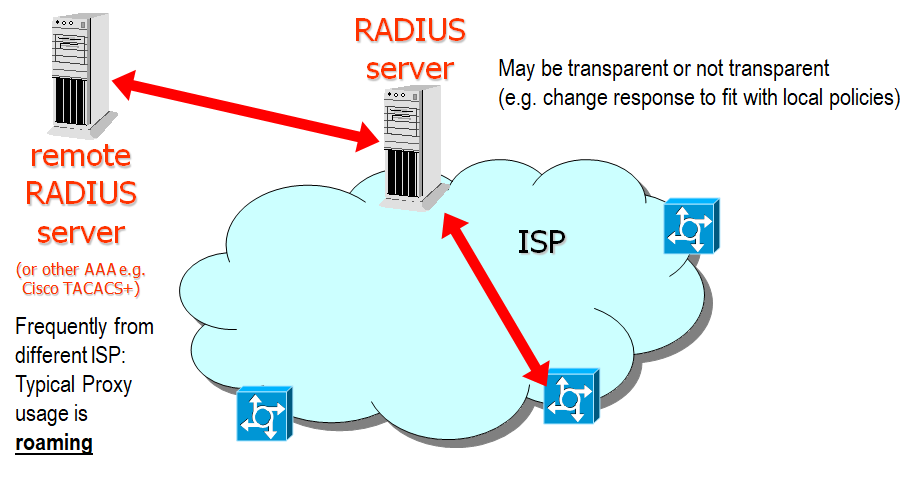
\includegraphics[scale=0.5]{proxyserver.png}
\end{center}
\subsection{Architettura RADIUS}
\begin{itemize}
    \item Applicazione server RADIUS;
    \item Database utente registrato per ogni voce nomeutente contiene almeno:\begin{itemize}
        \item Informazioni di autenticazione (segreti);
        \item Metodi di autenticazione:
        \item Attributi di autorizzazione;
    \end{itemize}
    \item Database dei client:\begin{itemize}
        \item Client autorizzati a comunicare con il server;
        \item \textbf{Client Radius}$\neq$\textbf{END-USER}
        
    \end{itemize}
    \item Database accounting:\begin{itemize}
        \item Utilizzato frequentemente per autenticazione;
    \end{itemize}
\end{itemize}
\subsection{Caratteristiche di sicurezza RADIUS}
\begin{itemize}
    \item \textbf{Risposta} autenticata per pacchetto:\begin{itemize}
        \item si utilizza un segreto condiviso;
        \item Assenza di trasmissione del segreto, come nel CHAP;
        \item La risposta viene autenticata;
        \item è hash-based e non HMAC-based;
        \item si utilizza come funzione hash MD5;
        \item Chiave condivisa a bassa entorpia;
    \end{itemize}
    \item Trasmissione crittografata della password utente. La chiave viene utilizzata per l'autenticazione.
\end{itemize}
\subsection{RADIUS authenticad reply}
Occorre definire un modello di attacco che verrà riportato di seguito. L'obiettivo è quello di usufruire di un servizio anche se non se ne ha la facoltà. Inanzitutto sappiamo che il vero segreto lo conoscono l'end-user e il server RADIUS; mentre il client NAS e il server RADIUS condividono lo stesso segreto $S$.
\begin{center}
    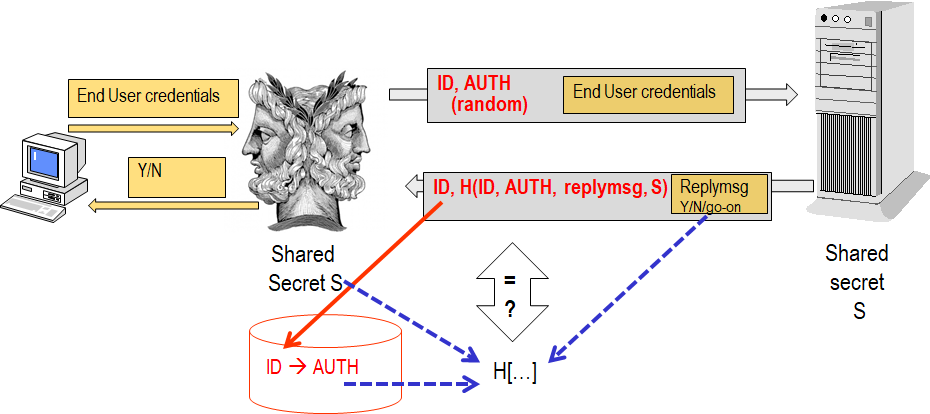
\includegraphics[scale=0.5]{AUTHREPLYRADIUS.png}
\end{center}
\begin{itemize}
    \item Il \textbf{NAS} parla con:\begin{itemize}
        \item End-USer: invia le sue credenziali;
        \item Server RADIUS.
    \end{itemize}
\end{itemize}
I passaggi sono i seguenti:
\begin{enumerate}
    \item  L'user invia le credenziali al NAS;
    \item crea un \emph{RADIUS alfy packet} contenente le credenziali dell'utente contenente ID e AUTH(Challenge randomica);
    \item il client NAS manda il paccheto al server che a sua volta risponde con \emph{$ID,H(ID,AUTH,replymsg,S)$} ed il messaggio di risposta che può essere \emph{Y/N/go-on}.
\end{enumerate}
Il campo ID serve a riconosce tramite un numero univoco il pacchetto in questione.
\begin{remark}
Questo schema può essere considerato come un challenge-response. In cui:\begin{itemize}
    \item Challenge è l'autenticatore della richiesta;
    \item La risposta include (e quindi convalida) il messaggio di risposta.
\end{itemize}
\end{remark}
\subsection{Formato del pacchetto RADIUS}
Il pacchetto RADIUS è formato da:\begin{center}
    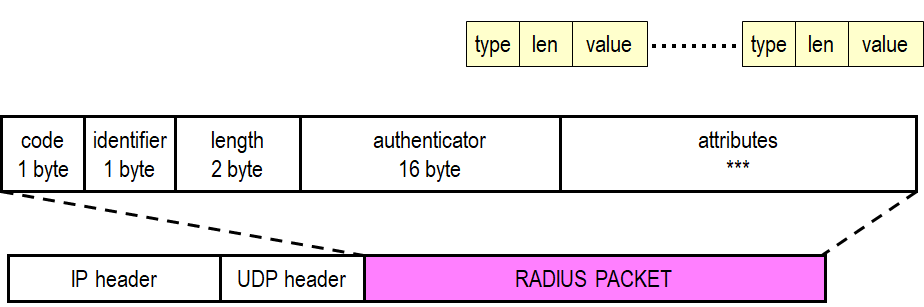
\includegraphics[scale=0.4]{packetFormat.png}
\end{center}\begin{itemize}
    \item \textbf{codice}: rappresenta il tipo di pacchetto RADIUS.\begin{center}
        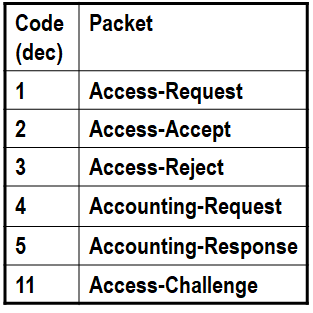
\includegraphics[scale=0.4]{codesRADIUS.png}
    \end{center}
    \item \textbf{Identificatore}: permettere di trovare una corrispondenza tra le richieste e le risposte;
    \item \textbf{Lunghezza}: lunghezza del pacchetto. Minimo 20 massimo 4096;
    \item \textbf{Autenticatore}: utilizzato per autenticare le risposte dal server e usati anche come nonce per la cifratura della password;
    \item \textbf{attributi}: campo informativo estensibile di circa 256 tipi. Il loro ordine non conta e si possono ripetere.
\end{itemize}
\subsection{Authentication Field}
\begin{itemize}
    \item \textbf{Access-Request(C$\rightarrow$ S)}: 16 byte generati casualmente. Quindi, imprevedibile e unico per evitare il replay attack;
    \item \textbf{Pacchetto di risposta(S$\rightarrow$ C Accept/Reject/Challenge)}:\begin{itemize}
        \item ID della richiesta;
        \item Autenticatore della richiesta;
        \item Segreto condiviso;
        \item Informazioni sulla rispsota del pacchetto: response packet è firmato. In caso contrario la risposta del server potrebbe essere falsificata.
    \end{itemize}
    \item $MD5(CODE|ID|Length|RequestAuth|Attributes|Secret)$
\end{itemize}
\subsection{Access-Request}
L'\textbf{access-request} tipicamente contiene:\begin{itemize}
    \item L'username\textbf{obbligatorio}: è la chiave di ricerca per accedere al database dell'utente;
    \item Password:\begin{itemize}
        \item User Password;
        \item CHAP-password (se si utilizza CHAP);
    \end{itemize}
    \item Identificatore dle client RADIUS:\begin{itemize}
        \item NAS-IP o NAS-Identifier: utile per accedere solo in un sottoinsieme di NAS;
    \end{itemize}
    \item Identificatore della porta al quale l'utente sta accedendo:\begin{itemize}
        \item NAS-Port se il NAS ha le porte. Pososno essere logiche (es.WiFi) o fisiche (es. Dial Up).
    \end{itemize}
    Vi è la possibilità che l'utente non sia abilitato all'accesso su specifiche porte.
\end{itemize}
\subsection{Password Encryption}
\begin{center}
    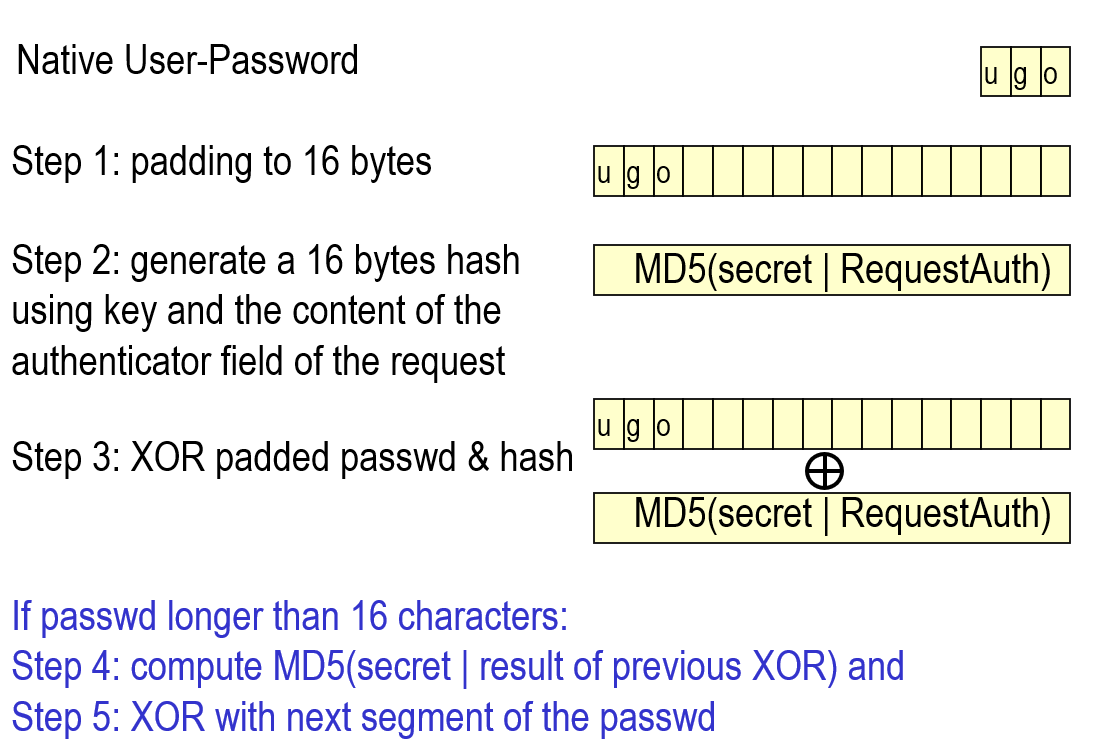
\includegraphics[scale=0.4]{passwordEncry.png}
\end{center}
\subsection{Access-Accept}
RADIUS come ulteriore tecnica di protezione utilizza il password encryption. In particolare, l'utente invia al NAS username e password e quest'ultimo lo invia al server. Dato che la rete fra il NAS e il server RADIUS non è sicura occorre criptare il messaggio.\newline
A tale scopo, si prende la password e la si padda fino a 16 byte, si prende questo blocco, lo si affianca al NONCE e si applica la funzione di hash MD5. Al risultato di questa operazione si applica l'operazione di XOR con la password. Infin, il risultato dello XOR viene inserito nel campo attributi del pacchetto RADIUS ed inviato.\newline
Nel caso in cui la password dell'utente sia pi+ lunga di 16 bytes, essa viene segmentata in blocchi di 16 bytes ciascuno (l'ultimo di questi blocchi, se minore di 16 byte, viene paddato fino al raggiungimento della dimensione richiesta). I singoli blocchi vengono quindi inseriti nella funzione hash M5D e si attua il procedimento canonico. La concatenzazione di questi risultati vengono inseriti nel campo attributo.
\begin{itemize}
    \item Risposta positiva del server: allora le credenziali di autenticazione dell'utente sono valide;
    \item Contiene tutta la configurazione delle specifiche del servizio tra cui un attribut del tipo di servizio e ulteriori parametri.
\end{itemize}
\subsection{Access-Reject}
L'accesso può essere rifiutato per due ragioni principali:\begin{itemize}
    \item Autenticazione fallita;
    \item 1 o più attributi nella richiesta di accesso non sono stati considirati accettabili.
\end{itemize}
\subsection{Access-Challenge}
La challenge per l'accesso viene utilizzato ogni qual volta che il server vuole un'ulteriore risposta dell'utente e può contenere:\begin{itemize}
    \item 1 o più attributo di reply-message;
    \item Testo mostrato all'utente;
    \item Esplicita challenge di autenticazione.
\end{itemize} Una Access-Challenge può essere il prompt di richiesta nome utente e password.\newline
Inoltre, il client NAS collezione le risposte dall'utente e le invia in una una richiesta di accesso.
\subsection{PPP CHAP supportato con RADIUS}
\begin{center}
    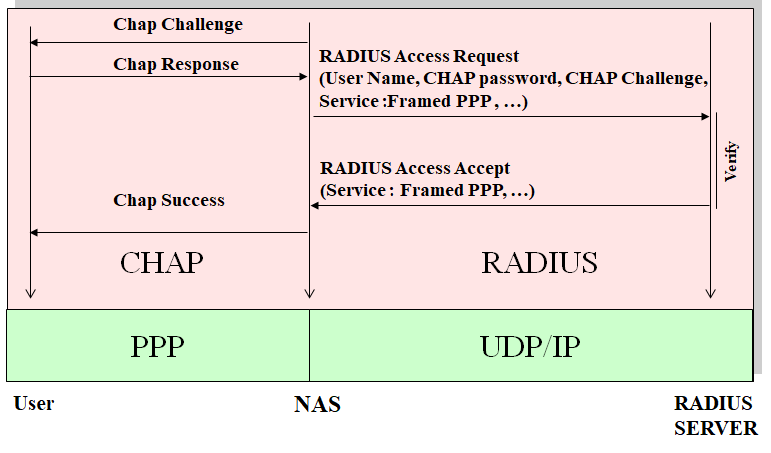
\includegraphics[scale=0.4]{PPPCHAPRADIUS.png}
\end{center}
Il collegamento punto punto \textbf{PPP} con CHAP può essere supportato con RADIUS. In particolare, la CHAP challenge viene generata localmente nel client NAS in assenza della password dell'utente. Inoltre, si invia la CHAP challenge con la risposta al server RADIUS. Quindi il client NAS, invia una \textbf{RADIUS Access-Request} al server RADIUS che dovrà verificare la correttezza delle credenziali fornitegli. Il Server RADIUS risponderà con un \textbf{Access-Accept} o \textbf{Access-Reject} in base alla validità o meno del pacchetto RADIUS. In caso affermativo, il client NAS notificherà all'utente che il PPP CHAP ha avuto esito positivo.
\begin{remark}
Nella comunicazione utente-NAS si utilizza PPP-CHAP.\newline
Nella comunicazione NAS-RADIUS server si utilizza UDP/IP.
\end{remark}
\subsubsection{Attack on PPP CHAP RADIUS Standard}
Lo schema di comunicazione appena proposto è lo standard effettivamente utilizzato nel mondo reale. Tuttavia, può essere attaccato con l'obiettivo di usufruire "a gratis" del servizio anche se non si ha l'autorizzazione nel farlo.\newline 
L'attacker si posizione in due punti della cominicazione: User-NAS e NAS-RADIUS Server. Questo permette di modificare le credenziali non valide che andrebbero al RADIUS Server (che porterebbe ad una risposta di tipo Access-Reject) in credenziali.\newline
In particolare, si compone di una prima fase in cui \textbf{l'attacker si pone fra User e NAS} si osservano le credenziali utente valide, salvandosi il seguente pacchetto:
\begin{center}
\begin{tabular}{ |c|c|c|c|c| } 
\hline
 Numero pacchetto & AUTH & Request & CHAP reply & CHAP Response\\
 \hline
\end{tabular}
\end{center}
Nella seconda fase, l'attacker si finge User,manda richiesta al NAS per essere autenticato. Il NAS invia la chap Challenge. A questo punto, l'attacker risponderà con credenziali arbitrarie e il NAS, una volta ricevuta la CHAP response, le invia al RADIUS Server. Tuttavia, \textbf{l'attacker si pone tra NAS e RADIUS Server}:lascia invariati i campi che vanno dal numero pacchetto al request (\emph{se vengono modificate, il RADIUS Server si accorgerebbe dell'attacco che sta avvenendo}), ma modifica il pacchetto RADIUS con le credenziali ottenute nella prima fase.Il server, quindi, verifica la validità delle credenziali, invia al NAS un RADIUS Access-Accept. Il NAS, una volta ricevuta risposta dal server notifica l'utente l'avvenuta autenticazione.\newline
L'attacker entra nel servizio "a gratis".
\subsubsection{Risuluzione}
Un modo per proteggersi da questo attacco è quello di autenticare tutti i campi del pacchetto o legare ogni richiesta di autenticazione alla risposta.
\begin{remark}
Come il prof. Bianchi insegna, si potrebbe risolvere utilizzando una copia della risposta nel RADIUS Client (NAS) ed inviare al RADIUS Server l'hash di $H(ID,AUTH,Replymsg,copia,S)$.
\end{remark}
\begin{remark}
L'ideale è quello applicare una funzione di hash a tutto.
\end{remark}
\subsection{RADIUS debolezze di sicurezza}
RADIUS è sensibile a message sniffing, poiché non vi è confidezialità, a message modification, poiché non c'è autenticazione per le richieste di accesso: ognuno può modificarne e crearne uno nuovo.
\subsubsection{Message-Authenticator}
L'autenticazione per le richieste di accesso può essere ottenuta tramite:\begin{itemize}
    \item \textbf{Message Authenticator}: per fornire la protezione dell'integrità per i messaggi di richiesta di accesso, viene aggiunto un tag a fine del messaggio di autenticazione detto \emph{authenticator} tra gli attributi del request packet. In aggiunta, quando si protegge il messaggio di richiesta di accesso con Message Authenticatori, si calcola un hash dell'intero pacchetto usando il segreto condiviso che condivide con il server RADIUS:$HMAC_MD5(Whole\ Packet)=HMAC-MD5(type|ID|len|RequestAuth|Attributes)$
    \item \textbf{EAP(Extensible Authentication Protocol)} Si tratta di un approccio arbitrario di autenticazione, ovvero di tecniche aggiuntive messe per la sicurezza di sistemi a cura di chi li realizza.
\end{itemize}
\subsubsection{Attack Shared Secret}
Le password scelte dagli utenti sono spesso a bassa entropia e spesso se ne utilizza una per tutte le reti (es. Fonera modem basati su RADIUS).
Per risolvere questo problema si prende un qualcosa di unico (che può essere un dato fisico di un device) e si fa in modo che il secret sia $HMAC(Secret,Dato\ Unico\ SEGRETO)$. Questa soluzione risulta scalabile e quindi ampiamente utilizzabile per le richieste di autenticazione.
Un tipico attacco al secret viene offerto dai cosiddetti \textbf{dictionary attack}.\begin{center}
    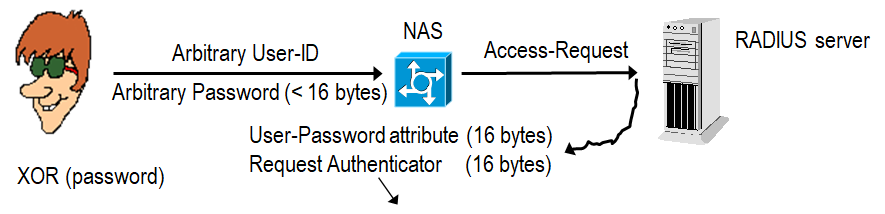
\includegraphics[scale=0.4]{dictionaryattackRADIUS.png}
\end{center}
Un attacker prende l'id di un utente, si presenta al NAS con una password a caso e ascolta la richiesta con l'obiettivo di capire quale elemento random è stato generato. Ascoltando la risposta acquisisce l'MD5 associato e, conoscendo la coppia richiesta-risposta, può entrare nel sistema.In particolare la richiesta gli fornisce la variabile causale ReqAUTH e la risposta RespAUTH (MD5). Questo accade perché l'attacker riesegue l'operazione di XOR con la sua password ottenendo l'MD5 della coppia. Quindi, conoscendo la challenge all'interno di MD5, l'unica cosa che gli rimane è il secret che otterrà effettuando un brute force attack. In realtà, non si necessità di una coppia, ma solo di una richiesta valida con la password ell'utente.\newline
Per evitare questo scenario, server un autenticatore di richieste unico e per realizzarlo si necessitano di 16 byte casuali ottenuti in questi modi:\begin{itemize}
    \item Attaccare fra loro diverse unità da 4  bytes pseudo-random:
    \item prendere una unità pseudo rando e paddarla finoa  16 bytes;
    \item effettuare MD5 dei 4 byte pseudo-random;
\end{itemize}
Valutando il ciclo di valori pseudo-random prodotti, mi permette di non avere ripetizioni. Tuttavia, il primo metodo è la peggiore soluzionepoiché generare 4 sequenze per volta fa in modo che is ricrea una sequenza già vista quattro volte più velocimente: si diminuisci il ciclo di ripetizione; il secondo e terzo hanno la stessa probabilità di ripetizione poiché si tratta sempre di 4 bit casuali che sono soggetti al paradosso del compleanno, ma comunque sempre migliori del primo.
\subsubsection{Replay Attack}
Nei replay attack in RADIUS, l'attacker si pone l'obiettivo di farsi autenticare/autorizzare senza una password valida.
\begin{center}
    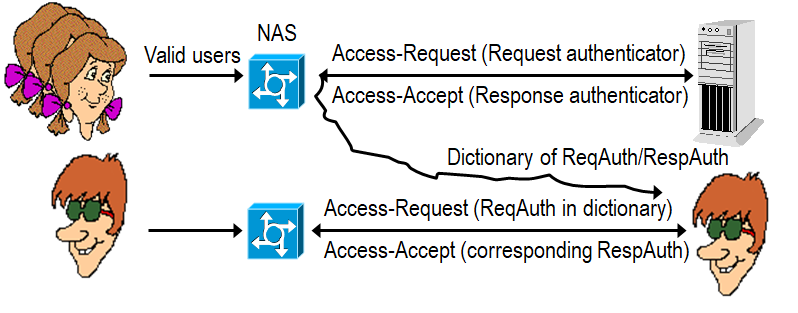
\includegraphics[scale=0.4]{replayRADIUS.png}
\end{center}
L'attacker può prendere la password di un utente tramite eavesdropping, cioè l'ascolto del traffico tra NAS e RADIUS Server. Così facendo, può costruire un dizionario ed effettuare un \emph{dictionary attack} per "breakkare" il cipher. Una volta conclusa questa fase, l'attacker effettua il replay attack al server con un login valido.
\begin{remark}
Il replay attack è un metodo di sfruttare i pacchetti catturati o reinviati all'utente causando un comportamento imprevisto o non voluto dal server. Nel caso in cui il server non riconosce il riuso dei dati e accetta ripetutamente i pacchetti trasmessi, l'attacco ha successo.
\end{remark}
\subsubsection{Attack User Password}
\begin{center}
    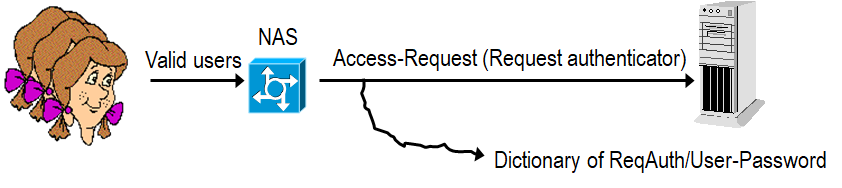
\includegraphics[scale=0.4]{attackpswRADIUS.png}
\end{center}
In questo tipo di attacco, l'attacker monitora passivamente il traffico di rete del NAS verso il RADIUS Server per costruire un dizionario compost da \textbf{request authenticator}\textbf{ReqAuth} a cui associa gli attributi della password utente. Assumendo che l'attacker può provare ad autenticarsi con una password nota ed infine catturare il pacchetto di Access-Request, si può effettuare l'operazione di XOR della porzione protetta della password utente con la password fornita al client NAS:\
\begin{equation*}
    (USR-PWD1)\bigoplus(USR-PWD2)=(PWD1\bigoplus MD5(secret,ReqAuth))\bigoplus(PWD2\bigoplus MD5(secret,ReqAuth))
\end{equation*}
\begin{equation*}
    =PWD1\bigoplus PWD2
\end{equation*}
Quindi, l'attacker può lanciare un brute-force attack offline per scoprire il segreto condiviso S. 
Un'altra alternativa è la seguente:
\begin{center}
    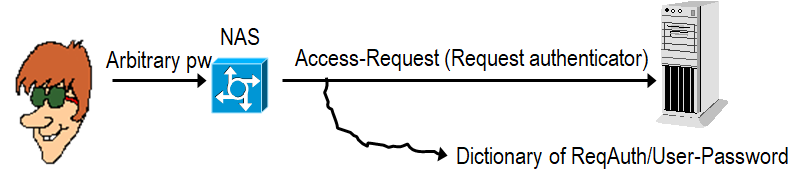
\includegraphics[scale=0.4]{attackpwdRADIUS.png}
\end{center}
In questo scenario, l'attacker invia attivamente delle password arbitario per formare un dizionario di password note e Access-Request. Quindi, se il server non impone un limite alle autenticazioni dell'utente, permette all'attacker di effettuare una ricerca esaustiva online per la password utente.
\subsubsection{Conclusioni}
Riassumendo, il protocollo RADIUS \textbf{non} è sicuro poiché:\begin{itemize}
    \item Se un hacker può monitorare dei tentativi di accesso, può costruire un database di coppie AUTH Request NONCE-Access Accept Packet (e quindi tentare un replay attack). Sarà a quel punto in grado di entrare nella rete quando il NAS genererà un access request nonce già usato. L'attacker potrà, allora, rispondere al NAS fingendosi server usando la risposta che aveva collezionato nel database. L'attacker si autentica da solo in quando conosce già la risposta che deve dare.
    \item Un altro modo è costruire una tabella dove ad ogni usare id si associano le informazioni password XOR MD5(secret,NONCE); alla ripetizione di una nonce, si effettua uno XOR per ottenere password1 XOR password2. A partire da queste due password legate da XOR è possibile, tramite un'opportuna analisi risalire alla password.
\end{itemize}
Un protocollo di livello applicatori non deve includere aspetti di sicurezza. Si può provare a sviluppare un proprio sistema di sicurezza, ma non è consigliato.
Considerando questi aspetti, RADIUS presenzt limitazioni funzionali dovuti a:\begin{itemize}
    \item \textbf{Scalabilità}: RADIUS usava UDP, protocollo non affidabile per migliaia di utenti. Pensando in ottica id un sistema esteso, in caso di crash di un server, a causa di UDP ci sarebbe packet loss su larga scala.\textbf{AAA server sono affetti da congestione e quindi perdita di pacchetti}. Utilizzare TCP, molto meglio;
    \item \textbf{Extendibility}:(type|len|value) per il tag non erano sufficienti per l'autenticazione. Questa idea adottata da RADIUS di utilizzare i suddetti byte negli attribuiti non fu abbastanz aper affrontare le nuove tecnologie. Questo portò ad una limitazione degli attributi utilizzabili;
    \item \textbf{Interoperability:} L'utilizzo di tanti server che adottano soluzioni differenti,crea consistenti problemi per l'interoperabilità-
\end{itemize}
\section{DIAMETER}
Il protocollo \textbf{DIAMETER} è un protocollo che nasce come evoluzione del protocollo RADIUS cercando di risolvere le sue problematiche. Questa tecnologia, insieme al RADext (estensione di RADIUS in assenza di sicurezza), è stata sviluppata da IETF (\emph{Internet Engineerign Task Force}). DIAMETER è tecnologicamente più avanzato ed è stato sviluppato in ottica Object Oriented Programming: il protocollo base è un protocollo di scambio di messaggi che poi si specializza nel settore in cui viene implementato.\begin{center}
    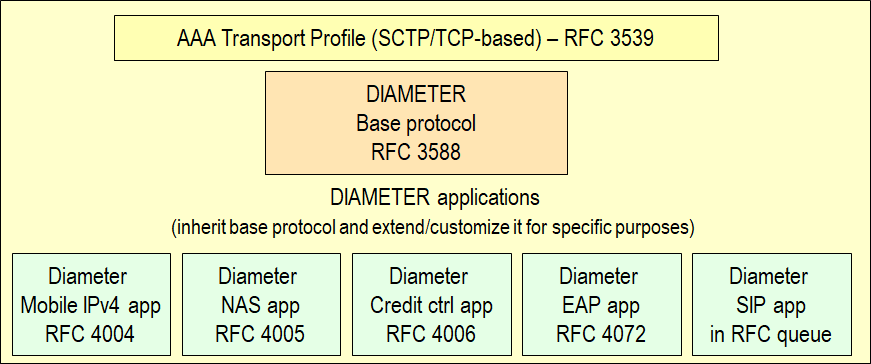
\includegraphics[scale=0.4]{DIAMETERALL.png}
\end{center}
\subsection{Catatteristihe}
Le caratteristiche che lo differenziano dal protocollo RADIUS sono le seguenti:\begin{itemize}
    \item DIAMETER non è un AAA protocol come il RADIUS, ma è un messaging protocol. In questo senso è detto protocollo Peer to Peer;
    \item AAA transport profile comunica come deve funzionare il trasposto dei messaggi che che nel caso di DIAMETER, non potendo utilizzare TCP come protocollo di trasposto (dato che garantisce l'arrivo in ordine dei pacchetti), si utilizza SCTP: protocollo TCP in cui si mantiene una connessione persistente tra clien e server e i pacchetti sono in pipeline su una connessione;
    \item Data la modularità di DIAMETER, dal protocollo base si sviluppano le varie derivazioni in base alla necessità;
    \item Al livello applicativo si hanno funzionalità di controllo degli errori e di ritrassmisione;
    \item Funzionalità di rilevamento di duplicati. (\emph{Fondamentale nelle funzioni di Accounting});
    \item Presenza dei cosiddetti \emph{watchdog}: pacchetti periodici che consentono di capire quando DIAMETER sta fallendo.
\end{itemize}
\subsection{Problemi TCP}
I problemi di TCP in questa specifica applicazione sono che:\begin{itemize}
    \item Strict Order Delivery e HOL;
    \item Mancanza di Multi-Homing;
\end{itemize} 
Quando richiesta, il NAS deve creare una connessione affidabile con l'AAA Server. Per garantirla, basta usare una connessione di tipo TCP. Una volta instaurata la connessione (Handshaking TCP), viene utilizzata per tutti i pacchetti successivi al primo. Ora, l'AAA server può usare più threads per gestire le richieste così che possano essere presi in carico diversi messaggi alla volta. Se un thread si ferma per un problema, TCP diventa svantaggioso in quanto grantisce l'ordine dei pacchetti: fa in modo che non si possa lavorare sui pacchetti successivi se non sono stati serviti i precedenti. Sarà quindi necessaria una nuova ricezione a partire dal messaggio perso.\newline Questa problematica viene detta \textbf{HOL(Head of the line blocking effect)},\newline
Per quanto riguarda il secondo problema: preso un NAS, se la rete fallisce si può garantire un servizio di continuità grazie a delle connessioni di ricambio ulteriori. Il problema è che l'IP è differenze, e siccome TCP si basa sulle socket che richiedono di pre-specificare l'IP, bisognerebbe creare una nuova socket ogni volta. Quindi, è necessario il \textbf{multi-homing} cioè la possibilità di avere più connessioni insieme in modo tale che se una fallisce se ne utilizzi un'altra.
\subsection{SCTP Stream Control Transport Protocol}
Si tratta di un protocollo che permetterebbe di avere multihominh, ma on viene utilizzato per il cosiddetto \emph{Chicken and egg problem e Internet Ossification}.\newline
Non molto tempo fa si utilizzava memorizzare i dati degli utenti su dispositivi, l'edge Network era quindi povero di dati. L'idea fu quella di portare i dati ai bordi della rete. Si utilizzarono i NAT per risolvere il problema degli indirizzi IP corti, al fine di connettere più device di quanti si poteva. Riguardo al DIAMETER non è possibile fare lo stesso discorso del NAT poiché, per renderlo reale, dovremmo porre due intermediari nella connessione fra due server. Se si utilizzasse un protocollo sconosciuto intermediario, esse bloccherebbero il traffico. Quindi, affinché sia possibile l'utilizzo di questo protocollo serve che i nodi di rete (intermediari fra due server) supportino SCTP,ma questo non accade.\begin{remark}
Nessuno può usare STCP poiché i nodi di rete lo bloccano e per far si che lo supportino si necessita che il protocollo venga utilizzato (\emph{Chicken and egg problem}). Questo problema ha portato all'\emph{internet ossification} ossia il blocco della crescita di Internet.
\end{remark}
\subsection{Miglioramenti DIAMETER rispetto a RADIUS}
\begin{itemize}
    \item \textbf{trasporto affidabile}: affidabilità essenziali per questioni monetari;
    \item \textbf{Standardized error and fail-over control}: al livello applicativo c'è il controllo degli errori e una serie di funzionalità di ritrasmissione gestita tramite l'invio di pacchetti che controllano se un device ha fallitO;
    \item\textbf{Peer Discovery, configuration,capability detection};
    \item \textbf{Supporto della comunicazione server client};
    \item \textbf{Gestione delle entità intermedie};
    \item\textbf{Estensione di limiti funzionali di RADIUS}:\begin{itemize}
        \item (Code|ID|Len|ReqAuth|Attr.) era la struttura del pacchetto di RADIUS. In DIAMETER venne adottato l'utilizzo di un header in quando non era chiaro l'ID assegnato ai pacchetti per via dei limiti funzionali legati alla tecnologia che era cambiata: adesso è possibile comunicare fra più server con i dovuti accorgimenti. DIAMETER modificò il tag di un header seguito da uno più \emph{AVPs}(attribute value pair).
        \begin{itemize}
            \item \textbf{Header(R|P|E|T)};\begin{itemize}
                \item R: specifica se si tratta di request o answer;
                \item P: indica se è proxabile;
                \item E:indica la presenza di errore;
                \item T: potentially retransmitting message, fa capire se il paccheto è uno che sto ritrasmettendo e non è nuovo.
            \end{itemize}
            \item \textbf{AVPs(V|M|P)};\begin{itemize}
                \item V: indica la presenza o meno dei dati vendor specific;
                \item M: Mandatory bit che serve in caso di diverse versioni fra NAS e Server che garantisce che un pacchetto non venga perso. Il server può richiedere di ritrasmettere perché non ha capito, risolvendo \textbf{l'interoperabilità}. Se M è impostato ad 1, allora il pacchetto deve essere rifiutato.
                \item P: dice se un messaggio è criptato o meno.
            \end{itemize}
 \begin{center}
     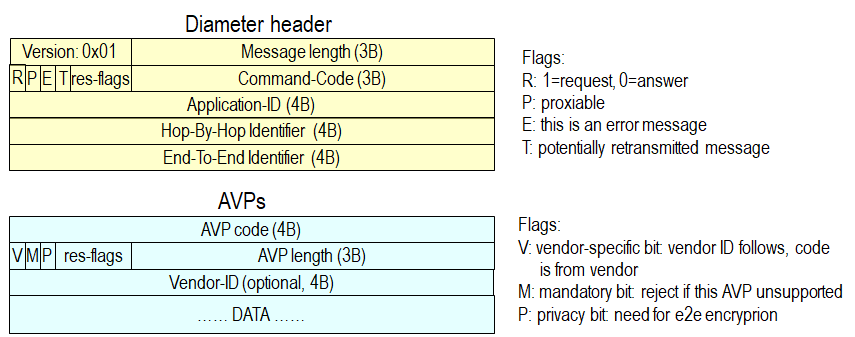
\includegraphics[scale=0.5]{DIAMETERPARAM.png}
 \end{center}
        \end{itemize}
    \end{itemize}
\end{itemize}
\subsection{Standardizzazioni DIAMETER}
\begin{itemize}
    \item Rely Agent;
    \item Proxy Agent;
    \item Redirect Agents;
\end{itemize}
In DIAMETER sono stati introdotti questi 3 agenti ntermediari che contengono i routing table per connettersi fra diversi server.\newline
Un \textbf{relay Agent} accetta le richieste e le indirizza al server corretto basandosi sulle informazioni contenuti nel messaggio; un \textbf{proxy agent} si comporta nella stessa maniera, ma può modificare anche i messaggi.
\begin{center}
    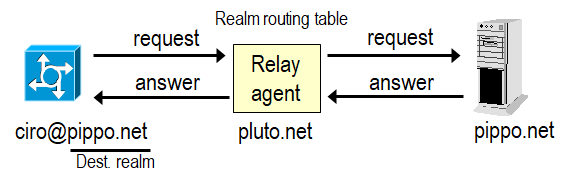
\includegraphics[scale=0.5]{relyAgent.png}
\end{center}

Preso un sistema di server, se uno crolla o cambia qualcosa, comunica il cambiamento a tutti gli altri. Anche quando qualcuno si unisce comunica con tutti. Questo discorso costituisce un incubo per la gestione poiché, se ci sono migliaia di server, è impossibile gestirli senza i \emph{relay e proxy agents}. Se si lasciano a loro le routing table se li gestiscono loro.\newline
Quindi,l'dea è quella di creare un controller centralizzato che non fa niente a parte mantenere le routing table. Ogni volta il serve, che ha il pacchetto da inoltrare, chiede al controller dove si trova il server a cui mandarlo. Così tutti il sistema risulta meno complicato in quanto le routing table sono centralizzate sul controller e tutti i server interrogano quello.\newpage
Infine il \textbf{redirect agent} non gestisce i dati, ma il controlla. Provvede alla routing decision sulle richieste in arrivo, ma non manda effettivamente la richiesta, ma solo il redirect. Ciò è utile quando le routing decision sono centralizzate. Il relay agent parla con il redirect agent.
\begin{center}
    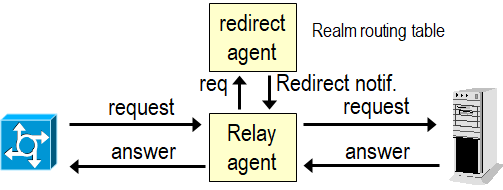
\includegraphics[scale=0.5]{redirectAgent.png}
\end{center}\newpage
\begin{center}
    \part{Second Midterm}
\end{center}
\section{Transport Layer Security}
\subsection{Introduzione}
TLS è un protocollo di livello di trasporto sicuro il cui progenitore è SSL v.3, Security Socket Layer. Da TLS v.1.0 ci furono nuove versione che inizialmente gradualemente: supportarono UDP (DTLS-\emph{Datagram TLS}), tolsero MD5/SHA-1 hash(TLS v1.2) e ammisero solamente AEAD\emph{(Authenticated Encryption with Associated Data)} (TLS v.1.3 -TLS completamente differente rispetto alle altre versioni).
In TLS v.1.3, disaccoppiarono il protocollo dall'algoritmo crittografico, cosa che fino a prima non era implementato.
\subsubsection{SSL/TLS: Visione stratificata}
\begin{center}
    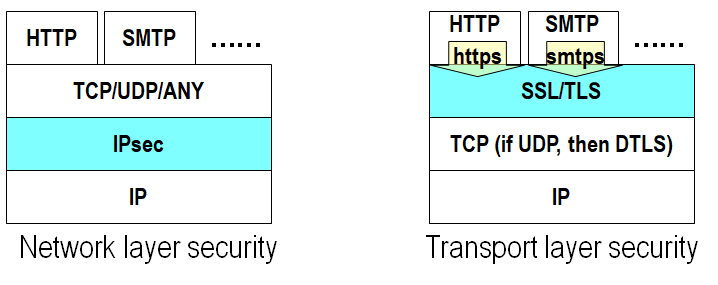
\includegraphics[scale=0.4]{SSL_TLS.png}
\end{center}
In IPsec proteggiamo l'intero pacchetto IP (Pacchetto IP, Payload, header) rispetto a dove sono destinati, sono utilizzati molto in telecomunicazione. \newline
Tramite l'utilizzo di TCP, possiamo scegliere di aprire una comunicazione crittografata o meno aprendo una socket protetta se necessario. Se vogliamo proteggere il canale di comunicazione, useremo TLS/SSL.\textbf{TLS protegge solo il payload TCP}: 
\begin{center}
\begin{tabular}{ |c|c|c|c|c| } 
\hline
 IP & TCP Header & \textbf{Protected TCP Payload}\\
 \hline
\end{tabular}
\end{center}
Questo perché se proteggessimo anche il pacchetto IP e il destination header, il router non saprebbe dove indirizzare il pacchetto. Quindi, con TLS vogliamo mantenere sia l'autenticazione e sia la cifratura dei dati.\newline
TLS, lavora tra il livello applicativo e il livello di trasporto e non protegge il protocollo TCP dato che il TCP Header può essere ancora modificato: si è soggetti a TCP spoofing.
\subsubsection{Application Support}
In TLS incapsularono male il pacchetto. In generale, l'incapsulazione corretta sarebbe stata che ogni protocollo specifica il contenuto del prossimo campo. Tuttavia, in TLS si riservarono porte diverse per diverse applicazioni ma nel caso in cui ci sono stessi servizi si utilizzano diverse porte. IETF hanno reso obsoleto questo metodo di incapsulazione.
IPsec, invece nell'IP packet vi è un campo protocollo che dice quello che sta dentro il prossimo campo, UDP.\newline
Stratificare correttamente aggiunge sicurezza al protocollo perché, per sapere che applicazione stai usando, devo prima sapere rompere IPsec dato che cifra l'intero pacchetto IP. Questo è un nuovo requisito di privacy detto \textbf{traffic flow confidentiality}.
\begin{center}
    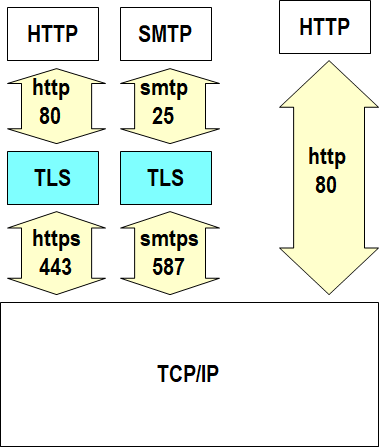
\includegraphics[scale=0.5]{TLSAPP.png}
\end{center}
\subsubsection{Obiettivi TLS}
Quando si progetta la sicurezza si deve pensare a due fasi:\begin{itemize}
    \item \textbf{Set-up l'ambiente}: quando si deve stabilire una sessione sicura bisogna pensare a quale algoritmo utilizzare, a come condividere il segreto e, se necessario, effettuare l'autenticazione.
    \item \textbf{Trasferire i dati dell'applicazione}: decidere come rendere la comunicazione privata (simmetric encryption) e mantenere l'integrità dei dati(HMAC).
\end{itemize}
In IPsec, questo processo è separato (IPsec IKE: Internet Key Exchange). In TLS, si effettuano queste cose in una: si ha una fase detta \textbf{handshake} in cui si negozia l'algoritmo da utilizzare, si crea il segreto condiviso e autenticare; la seconda fase è detta \textbf{record phase}.
\subsubsection{TLS Protocol Stack}
\begin{center}
    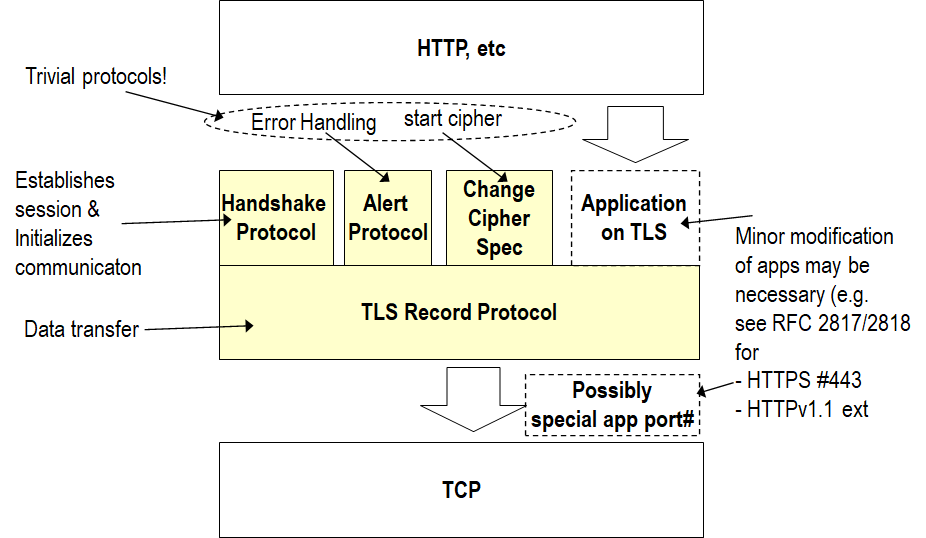
\includegraphics[scale=0.55]{TLSProtocolStack.png}
\end{center}
\textbf{TLS Record Protocol} contiene tutte le regole per gestire i pacchetti di TLS su cui si eseguono le applicazioni (\emph{Application on TLS}) deciso preliminarmente in TCP, il protocollo Handshake per configurare la rete e Alert Protocol per ricevere feedback dalle azioni che si eseguono.
\subsection{TLS Record Protocol}
\subsubsection{Record Protocol Operation}
\begin{center}
    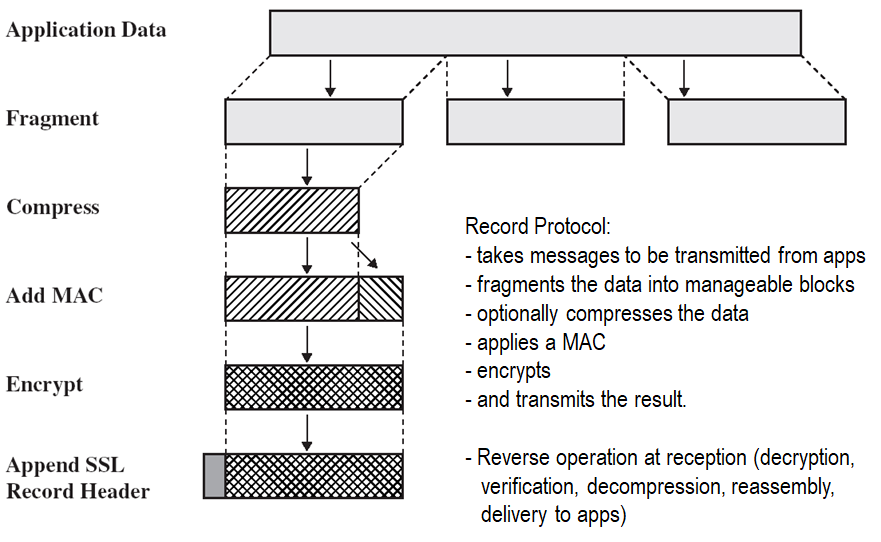
\includegraphics[scale=0.5]{RecordProtocolOperation.png}
\end{center}
Sono le operazioni da fare quando si è configurato il protocollo.
L'application data sono i dati ricevuti dal livello applicativo, si frammentano per facilitare il processamento. Per la sicurezza, dobbiamo comprimere,aggiungere integrità tramite HMAC e confidenzialità cifrando i dati. Intituivamente l'ordine di queste tre operazioni non dovrebbero mettere a rischio la sicurezza del protocollo. Tuttavia, non è così.\newline
La conseguenza di cifrare e poi comprimere è che il risultato prodotto dalla compressione non è più casuale ma è pseudo randomico e quindi è assolutamente da evitare. Un attacco detto CRIME si basa sulle azioni di compressione e poi cifratura per rompere TLS.\newline
Le operazioni di aggiungere il HMAC e poi cifrare sono assolutamente scorrette.
\newpage
\section{Message Authentication Code}
Per l'integrità di messaggio si utilizza HMAC \textbf{PRIMA DI TLS v.1.3}. Sappiamo che HMAC protegge da message spoofing e MITM. Per quanto riguarda il replay attack non siamo protetti. Alla fine delle 3 operazioni (compressione, aggiunta MAC e cifratura) si aggiunge un header detto Record Header formato nel seguente modo:
\begin{center}
    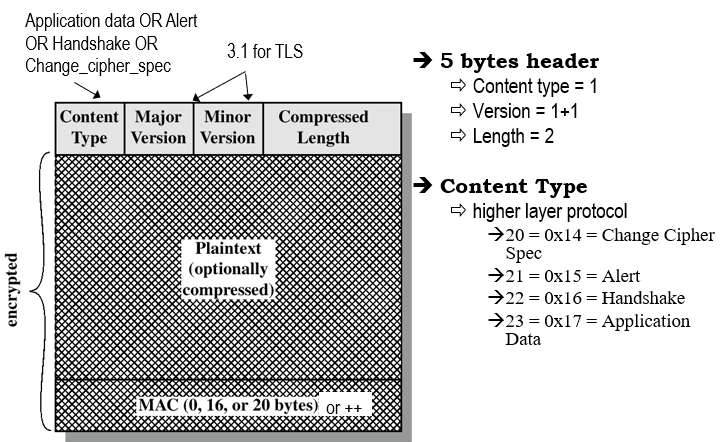
\includegraphics[scale=0.5]{TLS_Header.png}
\end{center}
Inoltre, sappiamo che per proteggerci da un ipotetico replay attack dobbiamo avere un Nonce, cioè una informazione che aggiunge freshness al messaggio cifrato e quindi che lo rende unico. TLS decise di adottare come NONCE il sequence number: quando si apre la connessione la connessione tra Client e Server si avvia una fase di negoziazione in cui si può decidere di iniziare con lo stesso numero di sequenza che indica il numero di pacchetto che si sta trasmettendo. Questo viene inizializzato a zero fino a $2^{64}$.\newline
\begin{center}
    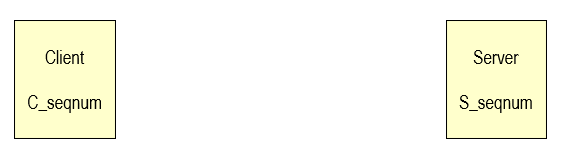
\includegraphics[scale=0.5]{SequenceTLS.png}
\end{center}
Per ottimizzare questa tecnica, dato che TCP permette la ricezione in ordine dei frammenti, si scelse di utilizzare lo stesso numero di sequenza utilizzato da TCP. La conseguenza di questa scelta è che hanno legato TCP a TLS e finché il protocollo di trasporto non cambia, tutto funziona. Nel caso di UDP questo non funziona da cui nasce la standardizzazione di DTLS.
\begin{center}
    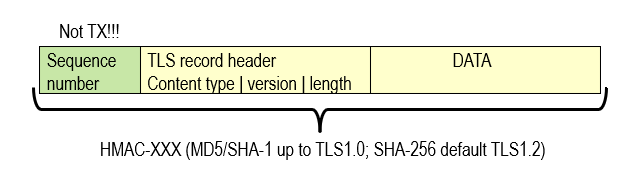
\includegraphics[scale=0.5]{SEQ2TLS.png}
\end{center}
Quindi, per aggiungere al messaggio integrità con HMAC e NONCE dobbiamo:
\begin{itemize}
    \item Prendere DATA;
    \item Affiancare il TLS record header;
    \item Aggiungere il NONCE (Sequence Number), ma questo non viene trasmesso, ma utilizzato nel calcolo di HMAC;
\end{itemize}
\subsection{Problematiche Encryption+Authentication}
Quello che vogliamo analizzare è il corretto modo di fare autenticazione e cifratura ed in particolare quali sono le problematiche a cui andiamo incontro.Ricordiamo che:\begin{itemize}
    \item \textbf{Integrità} protegge da:
    \begin{itemize}
        \item Message Spoofing: iniezione di messaggi;
        \item Message Tampering: modfica di messaggi;
    \end{itemize}
    \item Encryption non garantisce integrità finché non si utilizza AEAD.
\end{itemize}
\subsubsection{Combinare ENC+MAC}
\begin{center}
    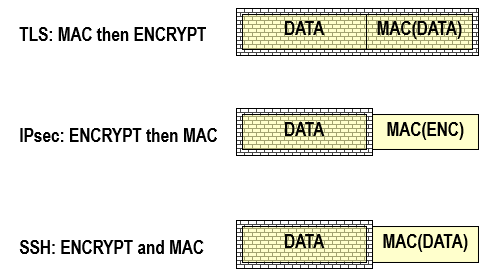
\includegraphics[scale=0.5]{ENCMAC.png}
\end{center}
Come abbiamo già visto possiamo avere la scelta di decidere quale operazione fra ENC e MAC precede l'altra:\begin{itemize}
    \item In TLS si scelse di effettuare prima l'integrità (MAC) e poi la confidenzialità (ENC): prendo il dato, calcolo il mac e poi cifro alla fine.
    \item IPsec scelse invece prima di prendere il dato, cifro producendo il CT e calcolo il MAC sul dato trasformato;
    \item In SSH scelse di prendere il dato cifrarlo e sul dato originario applicare il MAC. Queste operazione vengono svolte in parallelo.
\end{itemize} 
La soluzione più scorretta è la soluzione \textbf{ENCRYPT and MAC} (SSH). Dato che l'applicazione di ENC è la sicurezza semantica e l'utilizzo di MAC è la unforgeability dei messaggi, l'unione in questo ordine rompe la sicurezza semantica: l'utilizzo del MAC non garanstisce condifenzialità e, applicato al messaggio al plaintext, si potrebbero rilevare informazioni.
La soluzione di mezzo è quellaq di TLS: Mac and then Encrypt.
\section{Block Ciphers}
\begin{center}
    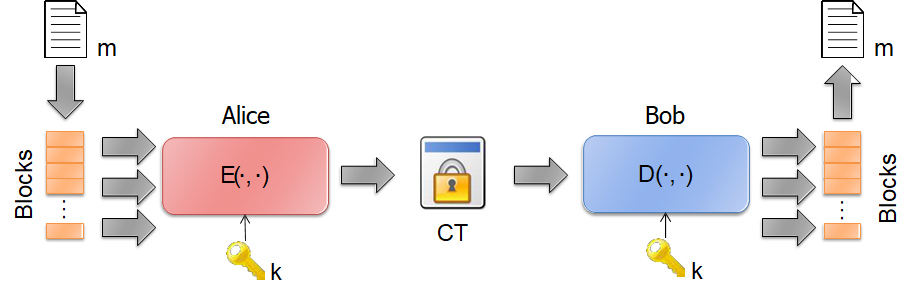
\includegraphics[scale=0.5]{blockCipher.png}
\end{center}
Una alternativa agli stream cipher sono i block cipher. I secondi sono la generalizzazione dei primi: 
\begin{itemize}
    \item Si prende il messaggio;
    \item Si divide il messaggio in blocchi di una certa dimensione;
    \item Si entra nel blocco \emph{E()} detto \textbf{pseudo random permutation block} che dipende dalla chiave k che effettua una permutazione dei blocchi formati al passo precedente. La chiave permette di selezionare una tra le $2^{KeySize}$ permutazione;
    \item Si produce il CipherText \textbf{CT};
    \item Per ottenere il PT, si applicare il blocco D() con le stesse caratteristiche di E();
    \item Si compattano i blocchi riordinati ed ottenuti al passo precedente;
    \item Si produce il PlainText \textbf{PT};
\end{itemize}
L'obiettivo è quello di generalizzare i substitution ciphers.
\begin{definition}[Pseudo Random Permutation]
Supponiamo $n=3$ abbiamo $|S|=2^n=8$ possibili uscite. Una permutazione è una funzione biettiva che mappa un elemento del dominio con uno del codomini: non si possono avere due elementi del dominio che vanno in uno del dominio.\newline
Tra tutte queste permutazioni, ne scegliamo una in maniera casuale (\textbf{uniforme}) ottenendo così, una delle $8!$ combinazioni possibili.
Quindi, formalmente:
\begin{equation}
    n:= numbero\ di\ bit \rightarrow 2^{n}!\ possibili\ permutazioni
\end{equation}
Tra queste permutazioni ne scegliamo una in maniera uniforme. Inoltre, la probabilità per cui in una permutazione non vi sono "fixed point", cioè che non ci sono due elementi che vanno in un solo output è di $\frac{1}{e}$
\end{definition}
\subsection{Problemi}
\begin{itemize}
    \item Cosa succede se il plaintext è più lungo della dimensione del blocco?
    \begin{center}
        \includegraphics[scale=0.5]{probl1.png}
    \end{center}
    Se la lunghezza del messaggio è maggiore del blocco, si divide il messaggio e si cifrano i blocchi in maniera indipendente. Questo metodo è detto \textbf{ECB}, ma è una applicazione di block cipher in maniera sbagliato poiché nel caso in cui si ha lo stesso PT si ha lo stesso CT e quindi viene a mancare la sicurezza semantica.\newline \textbf{ECB non deve essere mai utilizzato.}
    \item Cosa succede se cifriamo lo stesso messaggio due volte?
    \begin{center}
        \includegraphics[scale=0.5]{probl2.png}
    \end{center}
    Oltre a rimuovere le ripetizioni per gli stessi PT, dobbiamo risolvere il problema di cifrare lo stesso messaggio due volte e vogliamo avere un CT sempre differente. Data che la chiave è statica dobbiamo combinare al PT un fresh IV nel seguente modo:
    \begin{center}
        \includegraphics[scale=0.5]{IVblc.png}
    \end{center}
    \begin{itemize}
        \item Prendiamo PT della stessa dimensione del blocco e un IV TRNG;
        \item Effettuiamo lo XOR tra PT e IV per randomizzare e scegliere una delle permutazioni possibili;
        \item Applichiamo PRP con la chiave k per ottenere il CT;
        \item Si invia il CT e l'IV.
    \end{itemize}
    Per ottenere il PT:\begin{itemize}
        \item Prendo CT;
        \item Applico $PRP^-1$ con la chiave k;
        \item Applico XOR con il risultato prodotto al passo prima ed ottengo PT.
    \end{itemize}
    \textbf{IV non si deve mai ripete e deve essere non predicibile.}
\end{itemize}
\begin{remark}
\begin{itemize}
    \item \textbf{ECB} sipuò utilizzare se e solo se i messaggi sono più piccoli di un blocco e questi non si devono ripetere;
    \item Per messaggi ripetuti occorre utilizzare initialization vectors casuali e della stessa lunghezza del blocco;
    \item Per messaggi più lunghi del PT rispetto al blococ occorre applicare delle tecniche per combinare i blocchi deti \textbf{modes of operation}.
    \item Teoriacamente per avere uno schema semanticamente sicuro i passi da vare sono i seguenti:
    \begin{center}
        \includegraphics[scale=0.5]{semanticblc.png}
    \end{center}
    \begin{itemize}
        \item Si prende il mesaggio;
        \item lo si divide in blocchi;
        \item ad ogni blocco si affianca un IV generato da TRNG;
        \item Cifriamo indipendentemente i blocchi con il rispettivo IV;
        \item trasmettiamo ad ogni CT il proprio IV.
    \end{itemize}
    Questa soluzione non è pratica dato che si duplica la dimensione di memoria occupata rispetto all'input. Questo schema garantisce sicurezza semantica se tutti gli IV sono random e PRP è pseudo random.
\end{itemize}
\end{remark}
\subsection{Modes of Operation}
I modes of operation sono tecniche per combinare i block cipher per messaggi più lunghi di un singolo block. Vengono indicate con le tre lettere che posticipano AES-XYZ.\newline
I modi più utilizzati sono CBC \textbf{Cipher Block Chaining} e CTR \textbf{Counter Mode}; altri che sono stati standardizzati sono CGB \textbf{Cipher Feedback Mode} e OFB \textbf{Output Feedback Move}. Infine, i più avanzati GCM \textbf{Galois Counter Mode} e OCB \textbf{Offset Codebook Mode}.
\subsubsection{CBC- Cipher Block Chaining}
\begin{center}
    \includegraphics[scale=0.5]{CBC.png}
\end{center}
In questo mode of operation si utilizzare un IV casuale, si applica o XOR tra IV e il primo blocco, si ottiene il primo CT che fungerà da IV per il prossimo blocco e così via. L'uscita è pseudorandomica, ma cambiera in ogni messaggio dato che IV è casuale e non si ripete. L'unica operazione che bisogna fare una volta generati i blocchi CT, si affianca l'IV.\newline
L'overhead è diminuito alla lunghezza del messaggio con IV.\newline
La fase di decifratura avviene in parallelo. In particolare si prende il blocco CT, si applica l'inversa di PRP e poi si effettua lo XOR con il CT precedente ad eccezione del primo blocco in cui si utilizza l'initialization vector.
\begin{center}
    \includegraphics[scale=0.5]{CBCDec.png}
\end{center}
\begin{remark}
\begin{itemize}
\item Slow in encryption fast in decryption
    \item CBC è il mode of operation più utilizzato e sicuro se e solo se IV è casuale e non predicibile. Un attacco che ruppe questo schema è l'attacco \textbf{BEAST};
    \item La fase di cifratura e decifratura richiedono due circuiti, ma esistono altir modi come CTR,CFB,OFB che ne richiedono solo uno;
    \item Il PT deve essere un multiplo della dimensione del blocco: in caso di dimensione minore si padda fino alla dimensione del blocco con standard \emph{PKCS\#7}(\textbf{Public Key Crypto Standards}).
\end{itemize}
\end{remark}\newpage
Una problematica di avere un cifrario a blocchi concatentati è la presenza dei cicli: qualche permutazione, tramite il passaggio dal dominio e codominio per più volte, giunge allo stesso punto di partenza.
\begin{center}
    \includegraphics[scale=0.5]{ShortCycle.png}
\end{center}
In questo scenario, una chiave è detta debole se la corrispondente permutazione possiede un ciclo corto.
\begin{center}
    \includegraphics[scale=0.7]{CFBOFB.png}
\end{center}
\begin{center}
    \includegraphics[scale=0.7]{CFBOFBDec.png}
\end{center}
Per chiarire ulteriormente il problema dello short cycle occorre spiegare le seguenti modalità operative:
\begin{itemize}
    \item In CBF l'initialization vector viene trasformato e poi viene fatto lo XOR con il PT. La conseguenza è che l'output dopo il PRP è pseudo randomico che equivale al keystream di uno stream cipher. Il cuore della criptaggio non è più il PRP, come in CBC, ma è lo XOR. Abbiamo prodotto un algoritmo che per il primo blocco si usa un block cipher come uno streamcipher; da li in poi il CT viene utilizzato nel PRP e XORato con il PT. Al contrario, nella fase di decifratura, non abbiamo bisogno della trasformazione inversa, ma solamente utilizzare il blocco PRP in maniera diretta e poi effettuare lo XOR con CT. Abbiamo ridotto il circuito da 2 a 1. Caratteristiche:\begin{itemize}
        \item Non parallelizzabile:
        \item Cifratura lenta, decifratura veloce
    \end{itemize}
    \item La modalità di cifratura di OFB è simile a CFB con la differenza che si utilizza l'IV nel PRP, il suo risultato sarà il nuovo IV per il blocco successivo e poi successivamente viene effetuato lo XOR con PT. Si utilizza un block cipher come uno stream cipher. L'operazione di criptaggio non è più PRP, ma l'operazione di XOR. La costruzione diventa parallelizzabile ed è più robusta agli errori..
\end{itemize}
\begin{remark}
Usare un block cipher per generare un keystream è una pessima idea per la presenza degli "short cycle". Infatti, in base dal punto di partenza abbiamo delle ripetizioni: qualche IV può essere debole.
\end{remark}
\subsubsection{Counter Mode - CTR}
\begin{center}
    \includegraphics[scale=0.6]{CounterMOde.png}
\end{center}
CTR è un mode of operation molto veloce e segue i seguenti passaggi:
\begin{itemize}
    \item Inizializza un contatore ctr, e aumentato in ogni blocco;
    \item Cifra il counter con PRP (128bit), l'output è pseudo random :
    \item effettua lo XOR con l'elemento al passo precedente e il blocco PT;
    \item Effettua le operazioni per ogni blocco.
\end{itemize}
Nel caso in cui si ripete il criptaggio, si inizia dallo stesso numero. Tuttavia, dato che abbiamo 128 bit di IV (Counter) per i primi 96 bit(Nonce - Initial Counter Value) si ha un numero casuale e i restanti sono utilizzati come counter. 
Le principali caratteristiche sono le seguenti:\begin{itemize}
    \item cifrare e decifrare in parallelo;
    \item block cipher in una modalità stream cipher;
    \item cifrare/decifrare un blocco a nostra scelta(\emph{Random Access});
    \item assenza degli shot cycle perché per costruzione di PRP se l'ìnput è differente anche l'output è differente con in ciclo di $2^{n}$.
\end{itemize}
\subsection{BEAST Attack}
Il BEAST Attack sfrutta la predicibilità dell'IV nei CBC in TLS v.1.0/1.1. Durante l'invio di molteplici messaggi, con la stessa chiave, la condizione necessaria afifnché sia tutto sicuro è che l'IV deve essere diverso. Tuttavia questa condizione non è sufficiente perché l'IV deve essere anche non predicibile.
Infatti, se nell'invio dei messaggi, utilizziamo come IV l'ultimo blocco del messaggio precedente ci esponiamo a dei rischi.
\begin{center}
    \includegraphics[scale=0.4]{BEAST1.png}
\end{center}
Supponiamo che l'attacker sa che nel secondo blocco vi è la passsword che può essere una di due alternative. Se vale IND-CPA, allora questa informazione non dovrebbe creare problemi. Inoltre, ipotizziamo che l'attacker abbia visto l'ultimo CT del messaggio precedente, che possa predirre il prossimo IV e che possa criptare un messaggio a sua scelta (CPA). L'attacker può indovinare quello che vi è nel messaggio?\newline
L'attacker non può conoscere quale tra le due password sono state cifrate, ma può convincere l'implementazione a cifrare qualche dato di sua scelta.Challenge:\begin{center}
    \includegraphics[scale=0.4]{BEASTCHallenge.png}
\end{center}
\begin{itemize}
    \item Prendo newmsg[0] = IVpredicted XOR PAss XOR CT del blocco precedente;
    \item Effettuo lo XOR con la predizione che voglio fare così da cancellare l'IV;
    \item Se la predizione è andata a buon fine allora vedrò il CT che volevo predirre, altrimenti vedrò qualcos'altro.
\end{itemize}
Abbiamo rotto la sicurezza semantica.\begin{center}
    \includegraphics[scale=0.6]{BEASTIVPRED.png}
\end{center}
Questo attacco non è molto pratico perché:\begin{itemize}
    \item Occorre avere un agente in esecuzione sul browser;
    \item L'attacker deve effettuare injection di PT scelto;
    \item Deve essere flessibile alle moderne tecnologie;
    \item Se un attacker riesce a soddisfare i primi  3 punti deve effettuare comunque sia un brute force attack: AES blocchi da 128bit $\rightarrow 2^{123}$ guesses anche se si tratta di cookies di autenticazione la complessità è troppo elevata.
\end{itemize}
\subsubsection{Chosen Boundary Attack}
Sono attachi lineari rispetto la dimensione del messaggio. Si può iniettare qualcosa prima del messaggio e farlo cifrare e, sapendo a priori la posizione del messaggio, fanno corrispondere la prima lettera del messaggio all'ultimo blocco del bit. Ora, effettuanod un brute force attack posso indovinare la prima lettera della password e così via fino ad indovinare la password. La complessità è $256*N$.
\begin{center}
    \includegraphics[scale=0.5]{CBA.png}
\end{center}
\section{TLS Encryption}
TLS non supporta uno specifico cipher, ma è aperto a numerosi cipher.Ciò implica che si può integrare un buon cipher o pessimo; tuttavia gli attacchi sono presenti a prescindere dalla bontà del cipher. \newline
Iniziamo ad analizzare i possibili attacchi a TLS con cipher CBC.
\subsection{MAC-Then-Encrypt: CBC Padding Oracle Attack}
L'attacco Padding Oracle a CBC è un attacco che appartiene alla categoria \textbf{chosen cipher text attack-CCA}: l'attacker ha l'abilità di produrre un cipher text modificato e consegnarlo ad un oracolo per decifrarlo. Questi attacchi sono più pratici perché non vi è necessità di fare injection nell'utente.
\subsubsection{CBC Padding}
\begin{center}
    \includegraphics[scale=0.4]{CBCPADDING.png}
\end{center}
Il modo in cui paddiamo il payload segue la standardizzazione di \textbf{ PKCS\#7}: 
\begin{itemize}
    \item nell'ultimo blocco si ha l'ultimo byte in cui si inserisce la dimensione del padding (\emph{per sapere, nel decrypt, devo sapere quanto levare dal messaggio}),
    \item I byte precedenti sono di padding con valore uguale a quella specificata nella dimensione del padding \textbf{len}.
\end{itemize}
\begin{remark}
Il Padding non è ristretto alla dimensione di un singolo blocco ma è possibile anche prendere più di un blocco.
\end{remark}
Il vantaggio di questa tecnica è che può essere un modo per rilevare gli errori dato che la lunghezza definisce il valore dei byte precedenti a lui.
\subsection{CBC Decryption Steps}
La decription in CBC segue i seguenti passi:\begin{itemize}
    \item Decifra, finché il numero di byte non sono un multiplo della dimensione del blocco, ritorna un alert message decryption failed;
    \item Rimuovi il padding:\begin{itemize}
        \item Leggi l'ultimo byte per sapere la lunghezza;
        \item controlla e rimuovi gli ultimi L byte;
        \item Se il pad non è valido, ritorna un alert message decryption failed;
    \end{itemize}
    \item Controlla il MAC sul messaggio decifrato: se fallisce ritorna un alert message Bad\_record\_mac;
\end{itemize}
Di norma, questi messaggi facilitano il troubleshooting, ma da un aspetto di sicurezza questo porta a delle problematica dato che si danno delle informazioni all'attaccante su cosa non sta funzionando: l'ideale sarebbe non dare spiegazione ai fallimenti.\newline
In TLS queste informazioni permettono di rompere l'encryption.
\subsubsection{Attaco a CBC}
\begin{center}
    \includegraphics[scale=0.4]{AttackDEC.png}
\end{center}
\begin{itemize}
    \item \textbf{Goal}: Decifrare un blocco i.e. C[1]
    \item \textbf{Attacker Ability}: l'attacker puòp effettuare chosen ciphertext attack: l'attacker selezione un messaggio di sua scelta e può vedere la risposta.;
    \item L'attacker quindi può vedere 2 risposte: decryption o integrity. (il terzo (HMAC) viene esculso perché per la proprietà di inforgiabilità dei messaggi la probabilità di creare un messaggio valido è molto molto bassa);
\end{itemize}
Se seleziono un messaggio arbitrario CT, e mi ritorna BAD\_record\_MAC significa ch iul messaggio è stato decifrato e l'ultima parte del messaggio ha un padding corretto: si trapelano informazioni sul messaggio. Questa proprietà viene detta \textbf{Padding Oracle}: qualcuno mi dice se un messaggio è valido o meno. Ricordando il decrypt di CBC:
\begin{center}
    \includegraphics[scale=0.4]{CBCDecrypt.png}
\end{center}
Come già detto vogliamo attaccare il blocco c[1],l'attacker può vedere l'intero messaggio e vuole ottenere M[1]. Inoltre, assumiamo che l'obiettivo è quello di sapere se in M[1] ci stanno due messaggi di cui conosco l'ultimo blocco. L'attacker può effettuare un dictionary attack per capire l'ultimo byte: taglio tutto quello che va oltre al blocco che voglio attaccare e metto nell'ultimo byte del blocco precedente:\begin{center}
    $C[0][LastByte]XOR"ByteDaindovinare"XOR"ByteDiPadding$
\end{center}
Tutto il resto rimane invariato:\begin{center}
    \includegraphics[scale=0.5]{STARTFROM.png}
\end{center}
ora, avviamo il decrypt ed effettuiamo lo XOR tra C[0] modificato e DEC(K,C[1]). Nel caso in cui si indovina, allora l'ultimo Byte viene cancellato dall'operazione di XOR e ne rimarrà solo il padding, indovinando così l'ultimo block. Altrimenti, mi uscirà un padding diverso e quindi non avrò indonvinato. A questo punto, posso provare ad indovinare i byte precedenti in maniera iterativa scoprendo tutta la password. La complessità è lineare con la dimensione del blocco.
\paragraph{Esercizio d'esame}
TLS-Padding Oragle attack- Assume a CBC-based block encryption scheme which usese block sizes of 4 bytes each. Assume that the attacker sees the following ciphertext comprising 6 blocks(hex notation): \begin{center}
    f1 aa 11 04 || 34 35 f1 20 || 07 07 07 07 || 73 73 73 73 || 65 61 fb 08 || 91 11 5f 10
\end{center}
Assume now that the server is vulnerable to a Padding Oracle attack, and assume that the fourth block contains a secret code which is either 01 01 01 01 or 02 02 02 02. Which Chosen ciphertext message should the attacker send to the server/oracle to as to determine the code?\newline
\paragraph{Svolgimento} 
\begin{itemize}
    \item Dividi il messaggio  e butta tutto i blocchi successivi a quell dell'attack.;
    \item modifica il blocco precedente in molti modi:\begin{enumerate}
        \item Modifica solo dell'ultimo byte:\begin{center}
            07 XOR MyGuess(01) XOR Padding Valido(00)
        \end{center}
        \item Modifica del byte e padding giusto: 07 XOR MyGuess(01) XOR PaddingValido(03)" 3 byte +len(03)"
    \end{enumerate}
\end{itemize}
 \begin{center}
    f1 aa 11 04 || 34 35 f1 20 || 07 07 07 07 || 73 73 73 73 
\end{center}
Metodi:\begin{enumerate}
    \item \begin{center}
        07 XOR 01 XOR 00 = 0111 XOR 0001 XOR 0000=00110=06
    \end{center}
    Ora posso mandare il messaggio\begin{center}
    f1 aa 11 04 || 34 35 f1 20 || 07 07 07 06 || 73 73 73 73 
    \begin{remark}
    Se mandassi  f1 aa 11 04 || 34 35 f1 20 || 06 06 06 06 || 73 73 73 73 sarebbe ancora una risposta valida questo perché il pattern è lo stesso di quello che voglio decifrare.
    \end{remark}\end{center}
    \item \item \begin{center}
        07 XOR 01 XOR 03 = 0111 XOR 0001 XOR 0011=0101
    \end{center}
\end{enumerate}
In conclusione, anche modificando gli alert message in BAD\_MAC non si risolve il problema dato che, per la presenza dei side channels e dato che le operazioni sono fatte in maniera sequenziale, il tempo di esecuzione dei passaggi per decifrare il messaggio danno informazioni su quale passaggio si sta fallendo. Analizzando questo tempo, si ritorna al caso precedente e quindi si rompe il sistema. Nella programmazione di questi algoritmi bisogna programmare in constant time.
L'unica soluzione accettabile è quella di effettuare Encrypt-then-MAC introducendo così i cosiddetti AEAD\textbf{ Authenticated Encryption With Associated Data}.

\section{CRIME ATttack:TLS Compression Leak}
L'attacco CRIME serve ad evidenziare che la compressione seguita dalla cifratura in TLS non è sicura. Questo attacco si applica ogni qual volta che si applica la compressione seguita dalla cifratura. 
\paragraph{IDEA:}Supponiamo che sappiamo che una password è una alternativa fra due alternative. Cifriamo la password dopo la compressione: quando effettuiamo la compressione andiamo a modificare il messaggio che, in base alla cifratura, possiamo far trapelare delle informazioni. Da queste considerazioni possiamo decifrare la password.\newline In particolare, supponiamo che la password non sia nota, ma l'attacker può vedere la dimensione del dato compresso e poi cifrare e può iniettare ripetutamente un plaintext a sua scelta nel plaintext e vedere la dimensione del risultato.(\textbf{Plain Text Inject Attack}) Se nella compressione ho dei pattern posso vedere la dimensione del CT diversa da quella in ingresso, indovinando al massimo una lettera.\newline
\subsubsection{Dettagli dell'attacco}
DEFLATE utilizza due sotto algoritim: Huffman coding, LZ77. Il secondo rimpiazza 3 o più caratteri ripetuti con puntatori di offset e dimensione. Per esempio:\begin{center}
    GIUSEPPE BIANCHI AND MARCO BIANCHINI   36B
\end{center}
In:\begin{center}
    GIUSEPPE BIANCHI AND MARCO (-18,7)NI   31B
\end{center}
\subsubsection{Attacker Injects Chosen Text}
Supponiamo che vogliamo attaccare la password dell'utente formato da:\begin{itemize}
    \item Header noto;\item segreto non noto
\end{itemize}
Tutto cifrato. Tuttavia, posso utilizzare la parte nota come "gancio" per iniettare ripetutamente un messaggio a me noto:\begin{itemize}
    \item Att\_input+[header+secret]
\end{itemize}
Ogni volta che si ripete la cifratura, l'attacker vede la lunghezza del risulato. In particolare si inietta un commento contenente l'header noto e la lettera che vogliamo indovinare. Ripetiamo questo procedimento finché la dimenisone del CT non diminuisce e quando ciò accade abbiamo indovinato la lettera della password. Questo tipo di attacco è lineare con la dimensione della password.
\section{Authenticated Encryption}
Encryption non garantisce confidenzialità ne integrità in qualche caso spceifico, ma protegge solo contro attacchi di eavesdropping. Abbiamo bisogno di authenticated encryption: cipher progettati per essere sicuri contro attachi attivi(tampering) (CCA-\textbf{Chosen Ciphertext Attack}) e garanire confidenzialità e integrità.
Per mostrare che gli attacchi attivi (tapering) possono rompere la confidenzialità, mostriamo i seguenti esempi:
\begin{itemize}
    \item Supponiamo che un utente vuole inviare un emssaggio al server e sappiamo che utilizza TCP/IP stack. Il server una volta decifrato il messaggio lo trasferisce alla socket appropriata. Inoltre, assumiamo che l'attacker può solamente ascoltare i messaggi in una porta differente e rubare i dati tramite backend. I dati sono cifrati e protetti e si utilizza un IPset Tunnel con solo AES-CBC encryption(\textbf{Block Cipher}). 
    Un attacker, per modificare la porta in cui si direzionano i dati verso se stessi, cambia l'IV del pacchetto TCP/IP cifrato con CBC inserendo: 
    \begin{center}
        IV\'=IV XOR DEST=Old\_Port XOR DEST=NEW\_PORT
    \end{center}
    \item Ipotizziamo che l'attacker possiede solo la'accesso alla rete e può solamente tamper con il cipher text. A questo punto l'utente, da un terminale, invia in CTR mode una lettera alla volta. Ognuna di queste lettere siano inviate con un singolo keystroke in un pacchetto TCP. Dato che TCP effettua il controllo dei pacchetti con l'ausilio del campo del pacchetto cksum che permette di capire se un pacchetto è ben formato o meno: pacchetto ben formato o problema di trasmissione.
    Questo, tuttavia fornisce delle informazioni all'attaccante: se il pacchetto è valido si riceve un ACK, altrimenti niente. Il protocollo TCP si comporta proprio come un padding oracle e quindi effettuare un CCA.
    In particolare:
    \begin{itemize}
        \item \textbf{Obiettivo}: Decifrare un pacchetto specifico;
        \item \textbf{Svolgimento}: Attacker crea molteplici copie del pacchetto dell'utente e ne effettua lo XOR:
            \begin{center}
                \begin{tabular}{|c|c|c|c|}
                    IP hdr & TCP hdr & cksum $\bigoplus$ t & D $\bigoplus$ s\\
                \end{tabular}
            \end{center}
            Con t,s scelti dall'attaccante. Da tutte le combineazioni di t,s si ottengono molte equazioni valide:
            \newline\(checksum(hdr,D\bigoplus s)=t\bigoplus checksum(hdr,D)\)\newline
            Da tutte queste eqauzioni è possibile ottenere il valore del checksum e della lettera digitata.
    \end{itemize}
\end{itemize}
La sicurezza semantica (CPA) non può garantire ne integrità ne confidenzialità. Occorre utilizzare:
\begin{itemize}
    \item Se i messaggi hanno bisogno di integrità e non di confidenzialità, allora si utilizza \textbf{MAC};
    \item Se i messaggi hanno bisogno di integrità e confidenzialità, allora si utilizza \textbf{Authenticated Encryption Modes}.
\end{itemize}
Lo schema AE (\emph{Authenticated Encryption}) è il seguente:
\begin{center}
    \includegraphics*[scale=0.8]{2021-11-21-21-02-14.png}
\end{center}
Il messaggio entra in un encryption block che prende come argomento il messaggio e la chiave, si produce il CT che include un tag
di dimensione comlessiva strettamente maggiore di PT. Al momento di decifrare il CT si utilizza lo stesso percordso al contrario.
Se il tag è valido si riceve il messaggio, altrimenti si riceve un messaggio \textbf{REJECT}.\newline
AE è sicuro se:
\begin{itemize}
    \item è semeanticamente sicuro sotto un CPA;
    \item Garantisce integrità del CT \textbf{Ciphertext integrity};
\end{itemize}
\subsection{Ciphertext Integrity}
Supponiamo di avere un challenger che possiede una chiave segreta e un avversario. Diamo la possibilità all'avversario di
scegliere un messaggio e mandarlo al challenger n volte. Il Challenger lo cifra n volte tramite la chiave producendo il CT
e invia all'avversario. A questo punto, l'avversario può prendere un messaggio differente da tutti quelli prodotti, lo invia
al challenger. Ora, ascolto la risposta del challenger: se la risposta è reject, allora il gioco è vinto; altrimenti no.\newline
Per provare la ciphertext integrity:\textbf{La probabilità di non essere reject deve essere trascurabile}\newline
\subsection{AE with Associated Data}
\begin{center}
    \includegraphics*[scale=0.8]{2021-11-21-21-23-35.png}
\end{center}
Nasce dall'esigenza di inviare pacchetti con porzioni cifrati o no. i.e. pacchetto TCP. Tuttavia vogliamo sempre garantire
integrità.\newline
Nel caso in cui non vi sono associated date $\rightarrow$ CCA-Suecure Encryption cioè tutto è cifrato. nel caso in cui non si
voglia avere dati cifrati, si utilizza secure MAC.
\subsection{Design AEAD}
Quali sono le scelte di design di AEAD\dots
\begin{itemize}
        \item \textbf{Struttura}: \begin{itemize}
        \item Due livelli: prima cifra e poi effettua MAC; i.e. \textbf{AES-GCM}
        \item Un livello: tutto in una volta i.e. \textbf{OCB}
         \end{itemize}
        \item \textbf{Performance}: \begin{itemize}
        \item Prima cifra poi MAC: soluzione lenta;
        \item Difficile da parallelizzare.
        \item \textbf{Streamibility}: cipher online ad una passata
    \end{itemize}
    \item \textbf{Requisiti funzionali}: Dobe appliace la parte di associazione dei dati.
    \item \textbf{Resistenza agli errori}: Quanto e come è robusto AEAD quando IV viene riusato.
\end{itemize}
\subsection{AES-GCM: Galois Counter Mode}
AES-GCM è un algoritmo AEAD che utilizza una struttura Encrypt-then-MAC. Nella parte encrypt si utilizza AES-CTR(Counter Mode),
nella fase di autentitcazione MAC: GHASH (Galoise Hash). GHASH non è una funzione di hash crittografica che si basa sulla moltiplicazione
di polinomi nel GF(Galua Field)($2^{128})$.\newline
\subsection{AES-GCM:GHASH}
GHASH non è una funzione di hash crittografica, ma appartiene alla famiglia \emph{universal hash function}. La sua costruzione si basa
sulla moltiplicazione polinomiale carry-less nel Galua Fielsd.
\subsubsection*{Costruzione}
\begin{center}
    \includegraphics*[scale=0.8]{2021-11-21-22-03-58.png}
\end{center}
Assumiamo di avere due blocchi di messaggi \(m[1]\),\(m[2]\), iniziamo da un IV casuale affiancato ad un contatore. IV|CTR entra nelle blocco
AES che cifra l'IV tramite la chiave K. Il suo risultato (keystream) viene XORato con il messaggio. A questo punto occorre effettuare la parte 
autenticazione. Dobbiamo ricordarci che la chiave deve essere differente dalla fase encryption, quindi prendiamo la chiave originale e cifriamo u
una stringa nota per produrre una chiave di autneticazione. Questo processo viene detto \textbf{keyderivation}.\newline
Procedendo, prendiamo il CT, gli applichiamo il blocco GM con la chiave appena derivata, e produciamo il digest che verrà messo in XOR con il 
prossimo CT a cui verrà applicato GM e così via. Se ci fermassimo a questo livello siamo soggetti a \textbf{expansion attack}.
\begin{center}
    \includegraphics*[scale=0.8]{2021-11-21-22-05-03.png}
\end{center}
Quindi, per proteggerci, scelgiamo di autenticare anche la lunghezza del messaggio: all'utlimo passo, aggiungiamo nella catena la lunghezza dei CT
producendo così il messaggio. Il lavoro ancora non è finito poiché non si utilizza una hash function crittografica, ma occorre anche autenticare 
S con chiave K, ottenendo nu vettore pseudo randomico) e ne viene fatto lo XOR con il risultato della hash. Da questa operazione, si ottiene il TAG.
\textbf{Auth TAG} è sicuro anche se GM non è una crypto algoritmo.
\subsection{Wegman-Carter MAC}
Il \textbf{WegmanCarter MAC} è un teorema che supporta la costruzione di AES-GCM dicendo che grantisce la sicurezza di AES-GCM anche se GM non è crypto.
Si utilizzano funzioni hash non crifttografiche perché le funzioni hash crittografiche sono generalmente lente.\newline
Ovviamente queste hash non crittografiche devono soddisfare alcune proprietà. Per effettuare MAC con una funzione di hash non crypto, si necessitano di 
due blocchei:
\begin{itemize}
    \item \textbf{Universal hash Function}:
        Sono una famiglia di funzioni hash:
        \begin{center}
            \(H_k(msg)\rightarrow\{0,1,\dots,m-1\}\)
        \end{center}
        Questa famiglia è \emph{universale} se è difficile per un attacker, che
        non conosce la chiave, trovare una collisione. L'output di queste funzioni non deve essere necessariamente pseudo-random.\newline
        \textbf{Companion Property}: Per ogni coppia \(x\neq y\), Prob(\(H_x(M)=H_y(M)\))\(\leq \frac{1}{m}\). Il che implica:
        \begin{center}
            \item Cambiare una chiave dovrebbe cambiare casualemente il disgest: la probabilità che si ripeta una collisione cambiando la chiave
            deve essere trascurabile;
            \item Non ci dovrebbe essere alcuna coppia di messaggi M1,M2 che ritornano lo stesso hash per chiavi differenti.
        \end{center}
    \item \textbf{Pseudo Random Function};
\end{itemize}
\subsubsection{Costruzione di WegmanCarter}
Un MAC sicuro può essere costruito da un UHF (\emph{Univerasal Hash Function}) e un PRF(\emph{Pseudo Random Function}) dalla costruzione:
\begin{center}
    \(UHF_{k1}(msg)+PRF_{k2}(rand)\)
\end{center}
\begin{center}
    \includegraphics*[scale=0.8]{2021-11-21-22-43-47.png}
\end{center}
\subsection{Conclusioni-Costruzione Finale}
Fino ad ora abbiamo visto la parte Authenticated Encryption e per quanto riguarda la parte Associated DATA, li insieriamo nella catena prima di
effettuar ela parte di autenticazione.
\begin{center}
    \includegraphics*[scale=1]{2021-11-21-22-46-55.png}
\end{center}
\subsection{Criticità GCM}
Nel caso in cui si riutilizza il nonce (IV), si breakka il sistema.
\begin{itemize}
    \item AES-GCM TAG: tag=\( GHASH_H(CT)\bigoplus AES_K(IV,0)\)
    \item tag1=\( GHASH_H(CT1)\bigoplus AES_K(IV,0)\)
    \item tag2=\( GHASH_H(CT2)\bigoplus AES_K(IV,0)\)
    \item \(tag1\bigoplus tag2\)=\( GHASH_H(CT1)\bigoplus GHASH_H(CT2)\)
    \item GHAHS è lineare nello XOR: un attacker può recuperare un auth key H e forgiare quasiasi messaggio, ma la chiave K rimane comunque segreta.
\end{itemize}
\section{TLS Handshake Protocol}
TLS è un protocollo 2 in 1: in ogni sessione si ha una fase di \textbf{handshake} in cui si impostano tutti i parametri di comunicazione e \textbf{record protocolo} in 
si inviano i dati applicando encryption.
\subsection{Handshake}
La fase di handshake è la fasa di negozaiazione inizilia e scambio di parametri. Questa fase si compone di:
\begin{itemize}
    \item Mutual Authentication;
    \item Accordo sugli algoritmi;
    \item Scambio di valori casuali;(\emph{Nonce})
    \item Scambio dei sgegreti o informationi per calcolare i segreti.(\emph{Public Key Cryptography})
\end{itemize}
La fase di ripresa della sessione: \emph{Re-Keying} cioè si aggiornano i segreti.
\begin{center}
    \includegraphics*[scale=0.8]{2021-11-22-14-35-06.png}
\end{center}
\subsection{Handshale:goals}
\begin{itemize}
    \item Negoziazione sicura di un segreto condiviso tramite crittografia asimemetrica. Non viene mai trasmesso in chiaro e derivato
    da parametri crittografici che sono stati scambiati;
    \item Autenticvazione opzionale per client e server
    \item Negoziazione affidabile: l'attecker non può inferferire nella comunicazione e influenzare/alterare il ritorno della negoziazione senza essere rilevato dal client/server.
\end{itemize}
\subsubsection{Downgrade Attack}
\begin{center}
    \includegraphics*[scale=0.8]{2021-11-22-14-46-59.png}
\end{center}
Se possiamo negoziare qualcosa e questo non è protetto , allora posso modificare la negoziazione. Ne è un esempio
il \textbf{Downgrade Attack}: l'inizializzazione non (\emph{Client Hello , Server Hello}) è in PT. Ora l'attackent può cambiare la
versione di SSL ad un a versione precedente. Quindi il server crede che si possa utilizzare solo la versione vecchia, convincendo anche 
il Client: abbiamo modificato il protocollo da utilizzare con tutte le sue vulnerabilità e messo a rischio la comunicazione.
\textbf{La negoziazione deve essere affidabile.}
\subsection{Handshake Messages}
\begin{center}
    \includegraphics[scale=0.6]{2021-11-22-14-56-02.png}
\end{center}
\begin{itemize}
    \item Prima fase di Handshake (\emph{Client Hello, Server Hello}) in cui ci si introduce per impostare i parametri da negoziare:
        \begin{center}
            \includegraphics[scale=0.7]{2021-11-22-15-01-49.png}
        \end{center}
        L'obiettivo in generale è creare una connessione TLS/SSL tra client/server impostando:\begin{itemize}
            \item Accordo sulla versione TLS/SSL;
            \item Definizione dell'ID della sessione;
            \item Scambio dei NONCES (timestamp+valori casuali);
            \item Accordo sugli algoritmi di cifratura;
            \item Accordo sull'algoritmo di compressione.
        \end{itemize}
    \item \textbf{Handake Goals:}\begin{enumerate}
        \item La negoziazione sicura dei segreti condivisi viene effettuata tramite:
        \begin{itemize}
            \item \textbf{Crittografia asimmetrica};
            \item  I segreti non sono mai trasmessi in chiaro e derivati dai parametri crittografici scambiati:
        \end{itemize}
        \item Si avvia una fase sull'algoritmo da selezionare. Un \textbf{Cipher suite} è composto da:\begin{center}
            \(TLS\_AAAAAAAAAA\_WITH\_BBBBBBBBBBB\_CCCCCCCCCCCCCC\)
        \end{center}
        In cui A è la chiave pubblica usata(\emph{handshake}), la B è quale algoritmo si utilizza quando si inizia a crittogravare e CV rappresenza l'hash per il controllo di integrità.
        Un esempio è \textbf{TLS\_RSA\_WITH\_NULL\_MD5}
    \end{enumerate}
\end{itemize}

\begin{tabular}{cc}
    \includegraphics[scale=0.6]{2021-12-02-15-48-45.png}&
    \includegraphics[scale=0.6]{2021-12-02-15-57-06.png}
\end{tabular}
\subsection{Crittografia Asimmetrica}
\begin{center}
    \includegraphics[scale=1]{2021-12-02-16-26-53.png}
\end{center}
La \textbf{Crittografia asimmetrica} è una oforma di crittografia dove la chiave usata per cripatre è deversa e indipendente rispetto a quella usata per decriptare.
Similmente alore stream cipher e block scipher, per decriptare si utilizza la stessa trasformazione dell'encryption al contrario.\newline
L'aspetto fondamentale è che deve essere impossibile capire la chiae di decryption a partire da quella dell'encryption.
\subsubsection{Proprietà della chiave asimmetrica}
\begin{itemize}
    \item Se si conosce \(K_{ENC}\) non si può risalire a \(K_{DEC}\);
\end{itemize}
Se la chiave pubblica è quella utilizzata per l'encrypt, allora tutti possono cifrare, ma solo una persona può decifrare.\newline
Quello che occorre fare è la seguente cosa. Ipotizziamo di voler inviare dei dati confidenziali al server attraverso una un canale protetto: il client invia una richiesta al server per trasmettergli i dati, il server risponde comunicando al client la sua
chiave pubblica. Quindi il client prende la chiave e i dati e li cifra: l'attacker, potendo solamente cifrare i dati (dato che la chiave di cifratura è pubblica), non può risalire al messaggio che è stato inviato.
Allo stesso tempo, il server può decifrare i messaggi poiché ha già salvato e messo in sicurezza la chiave privata precedentemente ricevuta.
\subsubsection{Crittografia asimmetrica o simmetrica?}
Entrambe le crittografie sono insicure/sicure e dipende dagli algoritmi utilizzati e dalla dimensione dele chiavi. Tuttavia, la crittografia asimmetrica è più flessibile dato che non necessità la precondivisione delle chiavi a costo di utilizzare protocolli più complessi gravando, di conseguenza,
sulle prestazioni computazionali di circa 4/5 ordini di grandezza più lento.
\end{document}